\documentclass{magnolia}

\magtex{tex_driver={pdftex},
        tex_packages={xypic}}
\magfiche{document_nom={Graphes},
          auteur_nom={François Fayard},
          auteur_mail={fayard.prof@gmail.com}}
\magcours{cours_matiere={python},
          cours_niveau={mpsi},
          cours_chapitre_numero={8},
          cours_chapitre={Graphes}}
\magmisenpage{misenpage_presentation={tikzvelvia},
              misenpage_format={a4},
              misenpage_nbcolonnes={1},
              misenpage_preuve={non},
              misenpage_sol={non}}
\maglieudiff{}
\magprocess

% Inconnu
% Découvert / Visité
% Fermé

\lstMakeShortInline[columns=fixed,language=python]|

\begin{document}
%BEGIN_BOOK
\hfill
\includegraphics[width=0.6\textwidth]{../../Commun/Images/python-cours-complexity}
\magtoc

\section{Graphe}

\subsection{Graphe non orienté}

\begin{definition}
On appelle \emph{graphe non orienté} tout couple $G\defeq\p{S,A}$ où
\begin{itemize}
\item $S$ est un ensemble fini non vide dont les éléments sont appelés
  \emph{noeuds}, ou \emph{sommets}.
\item $A$ est un ensemble de paires $\ens{x,y}$, où $x$ et $y$ sont deux éléments
  distincts de $S$. Ces paires sont appelées \emph{arêtes}, ou \emph{arcs}.
\end{itemize}
\end{definition}

\begin{remarques}
\remarque En pratique, l'arête $\ens{x,y}$ sera notée $x-y$ ou $y-x$. On utilisera aussi
  les notations $xy$ ou $yx$. Intuitivement, une
  arête $x-y$ permet de passer du sommet $x$ au sommet $y$ et du sommet $y$ au sommet $x$.
  Deux sommets reliés par une arête sont dits \emph{adjacents}. On appelle \emph{voisin}
  d'un sommet $x$ tout sommet adjacent à $x$.
\remarque Dans notre définition, nous nous sommes interdit les
  \emph{boucles}, c'est-à-dire les arêtes reliant un sommet à lui-même. Nous n'autorisons
  pas non plus le fait d'avoir plusieurs arêtes entre deux sommets. Les graphes
  s'autorisant de telles arêtes sont appelés \emph{multigraphes}.
\remarque Dans un graphe non orienté
  \[\abs{A}\leq \frac{\abs{S}\p{\abs{S}-1}}{2}.\]
\remarque Lorsqu'on parle d'un graphe à $n$ sommets sans préciser $S$, on prend
  $S\defeq\interefo{0}{n}$.
\end{remarques}

\begin{exemples}
\exemple Le graphe \emph{entièrement déconnecté} possède $n$ sommets et aucune arête.
  \begin{center}
  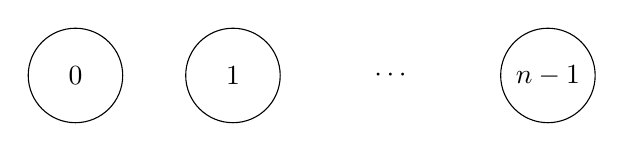
\begin{tikzpicture}
  \node[shape=circle,draw=black,minimum size=1.2cm] (0) at (0,0) {0};
  \node[shape=circle,draw=black,minimum size=1.2cm] (1) at (2,0) {1};
  \node[] (2) at (4,0) {$\cdots$};
  \node[shape=circle,draw=black,minimum size=1.2cm] (3) at (6,0) {$n-1$};
  \end{tikzpicture}
  \end{center}
\exemple Le graphe \emph{chemin} à $n$ sommets $\mathcal{K}_n$ possède une arête entre
  $i$ et $j\in\interefo{0}{n}$ si et seulement si $j=i+1$.
  \begin{center}
  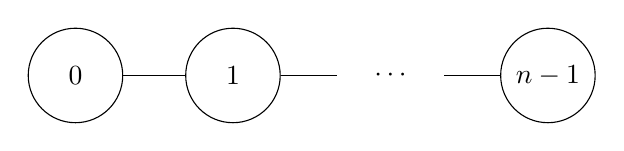
\begin{tikzpicture}
  \node[shape=circle,draw=black,minimum size=1.2cm] (0) at (0,0) {0};
  \node[shape=circle,draw=black,minimum size=1.2cm] (1) at (2,0) {1};
  \node[] (2) at (4,0) {$\quad\cdots\quad$};
  \node[shape=circle,draw=black,minimum size=1.2cm] (3) at (6,0) {$n-1$};
  \path [-](0) edge node[left] {} (1);
  \path [-](1) edge node[left] {} (2);
  \path [-](2) edge node[left] {} (3);
  \end{tikzpicture}
  \end{center}
\exemple Le graphe \emph{cycle} à $n$ sommets $\mathcal{C}_n$ (pour $n\geq 3$) possède une
  arête entre $i$ et $j\in\interefo{0}{n}$ si et seulement si $j\equiv i+1\ [n]$.
  \begin{center}
  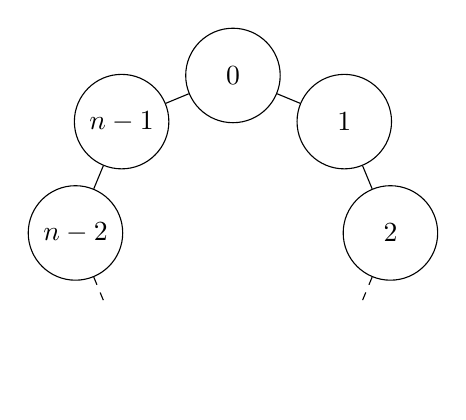
\begin{tikzpicture}
  \node[shape=circle,draw=black,minimum size=1.2cm] (0) at (0,2) {0};
  \node[shape=circle,draw=black,minimum size=1.2cm] (1) at (1.414,1.414) {1};
  \node[shape=circle,draw=black,minimum size=1.2cm] (2) at (2.0,0.0) {2};
  \node[shape=circle,draw=white,minimum size=1.2cm] (3) at (1.414,-1.414) {};
  \node[shape=circle,draw=white,minimum size=1.2cm] (4) at (-1.414,-1.414) {};
  \node[shape=circle,draw=black,minimum size=1.2cm] (5) at (-2,0) {$n-2$};
  \node[shape=circle,draw=black,minimum size=1.2cm] (6) at (-1.414,1.414) {$n-1$};
  \path [-](0) edge node[left] {} (1);
  \path [-](1) edge node[left] {} (2);
  \path [-,dashed](2) edge node[left] {} (3);
  \path [-,dashed](4) edge node[left] {} (5);
  \path [-](5) edge node[left] {} (6);
  \path [-](6) edge node[left] {} (0);
  \end{tikzpicture}
  \end{center}
\exemple Le graphe des utilisateurs de Facebook a un sommet pour chaque utilisateur
  et une arête entre deux sommets lorsque deux utilisateurs sont \emph{amis}. Notons que
  $\abs{S}$ est de l'ordre de $10^9$ et que $\abs{A}$ est de l'ordre
  de $10^{11}$, ce qui pose quelques difficultés algorithmiques.
\exemple Dans le graphe du métro parisien, les sommets représentent les stations de
  métro et les arêtes, les liaisons entre ces stations.
\begin{center}
  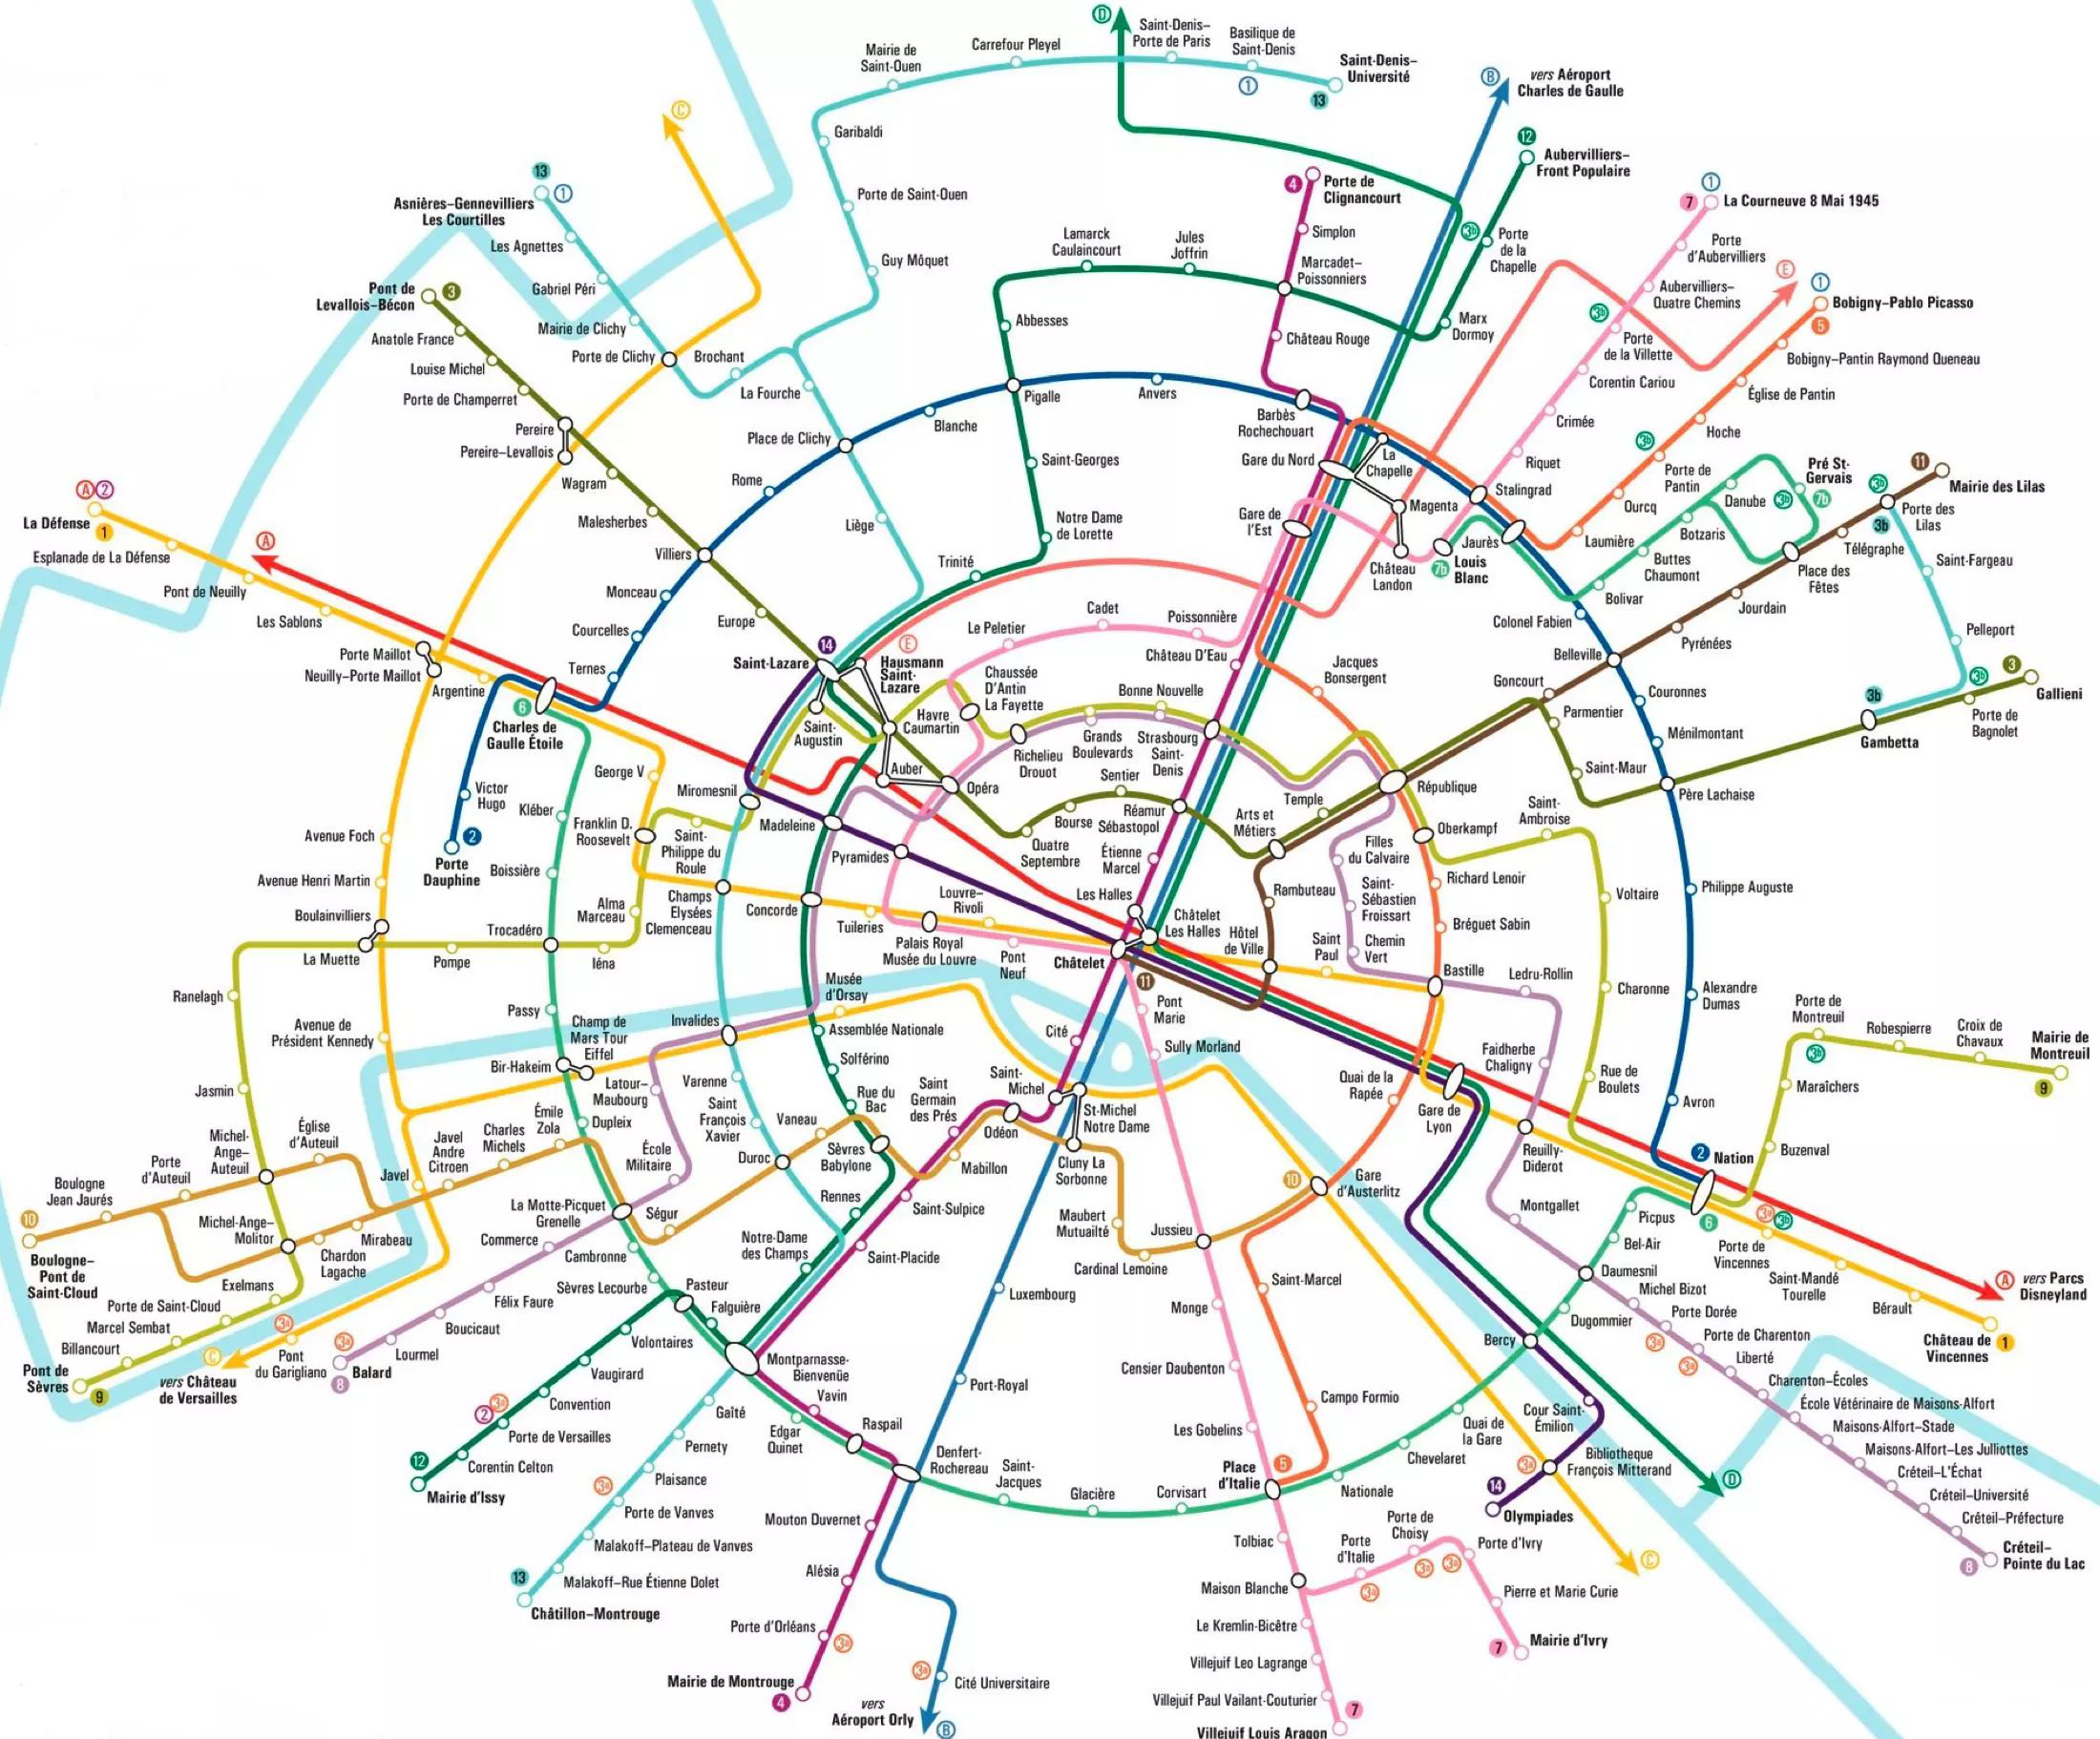
\includegraphics[width=0.8\textwidth]{../../Commun/Images/python-cours-metro-paris}
\end{center}
\end{exemples}


\begin{definition}
On appelle \emph{degré} d'un sommet $x$ le nombre d'arêtes de la forme $x-y$.
\end{definition}

\begin{remarqueUnique}
\remarque Le degré d'un sommet est son nombre de voisins.
\end{remarqueUnique}

\begin{definition}
On appelle \emph{chemin} de longueur $n$ toute suite $c\defeq z_0,z_1,\ldots,z_{n}$ de $n+1$ sommets telle que
\[\forall k\in\interefo{0}{n}\qsep z_k-z_{k+1}\in A.\]
Les sommets $z_0$ et $z_n$ sont appelés \emph{extrémités} du chemin et on dit que $c$
\emph{relie} $z_0$ à $z_n$. 
\end{definition}

\begin{remarques}
\remarque On peut aussi voir un chemin de longueur $n$ comme une suite de $n$ arêtes consécutives. Un chemin de longueur $n$ est constitué de $n+1$ sommets et de $n$ arêtes.
\remarque On accepte les chemins de longueur nulle, reliant un sommet à lui-même, sans arête.
\remarque Dans la suite, on notera $l(c)$ la longueur d'un chemin $c$.
\end{remarques}

\begin{definition}
Un chemin $z_0,z_1,\ldots,z_n$ est dit
\begin{itemize}
\item \emph{élémentaire} lorsqu'il ne passe pas deux fois par le même sommet, c'est-à-dire
  lorsque les sommets sont deux à deux distincts.
\item \emph{simple} s'il ne passe pas deux fois par la même arête, c'est-à-dire lorsque
  les arêtes $z_k - z_{k+1}$ sont deux à deux distinctes.
\end{itemize}
\end{definition}

\begin{remarqueUnique}
\remarque Tout chemin élémentaire est simple. Cependant la réciproque est fausse puisque
sur le graphe non orienté ci-dessous, le chemin $0-1-2-3-1-4$ est simple, mais pas
élémentaire.
\begin{center}
  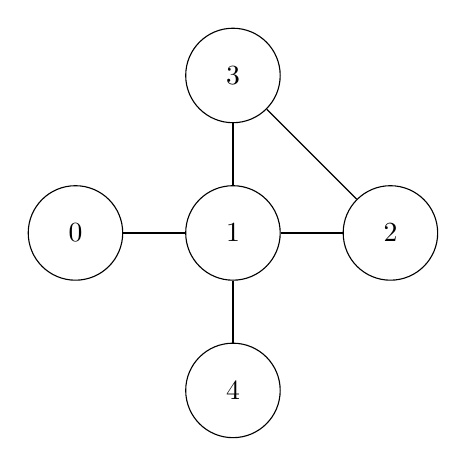
\begin{tikzpicture}
  \node[shape=circle,draw=black,minimum size=1.2cm] (0) at (-2,0) {0};
  \node[shape=circle,draw=black,minimum size=1.2cm] (1) at (0,0) {1};
  \node[shape=circle,draw=black,minimum size=1.2cm] (2) at (0,2) {3};
  \node[shape=circle,draw=black,minimum size=1.2cm] (3) at (2,0) {2};
  \node[shape=circle,draw=black,minimum size=1.2cm] (4) at (0,-2) {4};
  \path [-](0) edge node[left] {} (1);
  \path [-](1) edge node[left] {} (2);
  \path [-](2) edge node[left] {} (3);
  \path [-](3) edge node[left] {} (1);
  \path [-](1) edge node[left] {} (4);
  \end{tikzpicture}
\end{center}
\end{remarqueUnique}

\begin{definition}
Un sommet $y$ est dit \emph{accessible}
depuis un sommet $x$ lorsqu'il existe au moins un chemin
reliant $x$ à $y$.
\end{definition}

\begin{remarqueUnique}
\remarque Puisqu'on accepte les chemins de longueur nulle, tout sommet est
  accessible depuis lui-même.
\end{remarqueUnique}

\begin{proposition}
Dans un graphe non orienté, la relation d'accessibilité est une relation d'équivalence
sur $S$. 
\end{proposition}

\begin{remarques}
\remarque Si $y$ est accessible depuis $x$, alors $x$ est
  accessible depuis $y$. On dit alors que $x$ et $y$ sont \emph{connectés}.
\remarque On appelle \emph{composante connexe} toute classe d'équivalence
pour cette relation.
\end{remarques}

\begin{definition}
On dit qu'un graphe non orienté est \emph{connexe} lorsqu'il ne possède qu'une seule
composante connexe, c'est-à-dire lorsque tous ses sommets sont connectés.
\end{definition}

\begin{definition}
Si $y$ est un sommet accessible depuis un sommet $x$, on appelle distance entre $x$ et
$y$ l'entier
\[{\rm d}(x, y) \defeq \inf \ensim{l(c)}{c
      \textnormal{ est un chemin de } x \textnormal{ à } y}.\]
Un \emph{chemin de longueur minimale} de $x$ à $y$ est un chemin $c$
de $x$ à $y$ tel que $l(c) = {\rm d}(x, y)$.
\end{definition}

\begin{remarques}
\remarque Lorsque $y$ n'est pas accessible depuis $x$, la convention est de poser
  ${\rm d}(x, y)\defeq +\infty$.
\remarque Conformément à ce qu'on attend d'une distance
  \begin{eqnarray*}
  \forall x\in S,& & {\rm d}(x, x)=0,\\
  \forall x,y\in S,& & {\rm d}(y, x)={\rm d}(x, y),\\
  \forall x,y,z\in S,& & {\rm d}(x, z)\leq {\rm d}(x, y)+{\rm d}(y, z).\\
  \end{eqnarray*}
\end{remarques}

\begin{definition}
On appelle \emph{cycle} tout chemin simple de longueur non nulle dont les deux
extrémités sont identiques.
\end{definition}
  
\begin{remarques}
\remarque Dans la définition, il est nécessaire de se limiter aux chemins simples, sinon
  on pourrait construire des \og cycles \fg dans les graphes 
  en parcourant une même arête dans un sens puis dans l'autre.
\remarque Dans un graphe non orienté, la longueur d'un cycle est supérieure ou égale à 3.
\remarque Un cycle sera dit \emph{élémentaire} lorsque la seule répétition de sommets est celle de
  ses extrémités. Un cycle est élémentaire si et seulement si il ne contient pas
  d'autre cycle.
\item On dit qu'un graphe est \emph{acyclique} lorsqu'il ne possède pas de cycle.
\end{remarques}

\begin{exempleUnique}
\exemple Dans le graphe suivant, le chemin $4- 5- 6- 9- 8- 6- 4$ est un cycle. Ce graphe possède 4 cycles élémentaires.
\begin{center}
  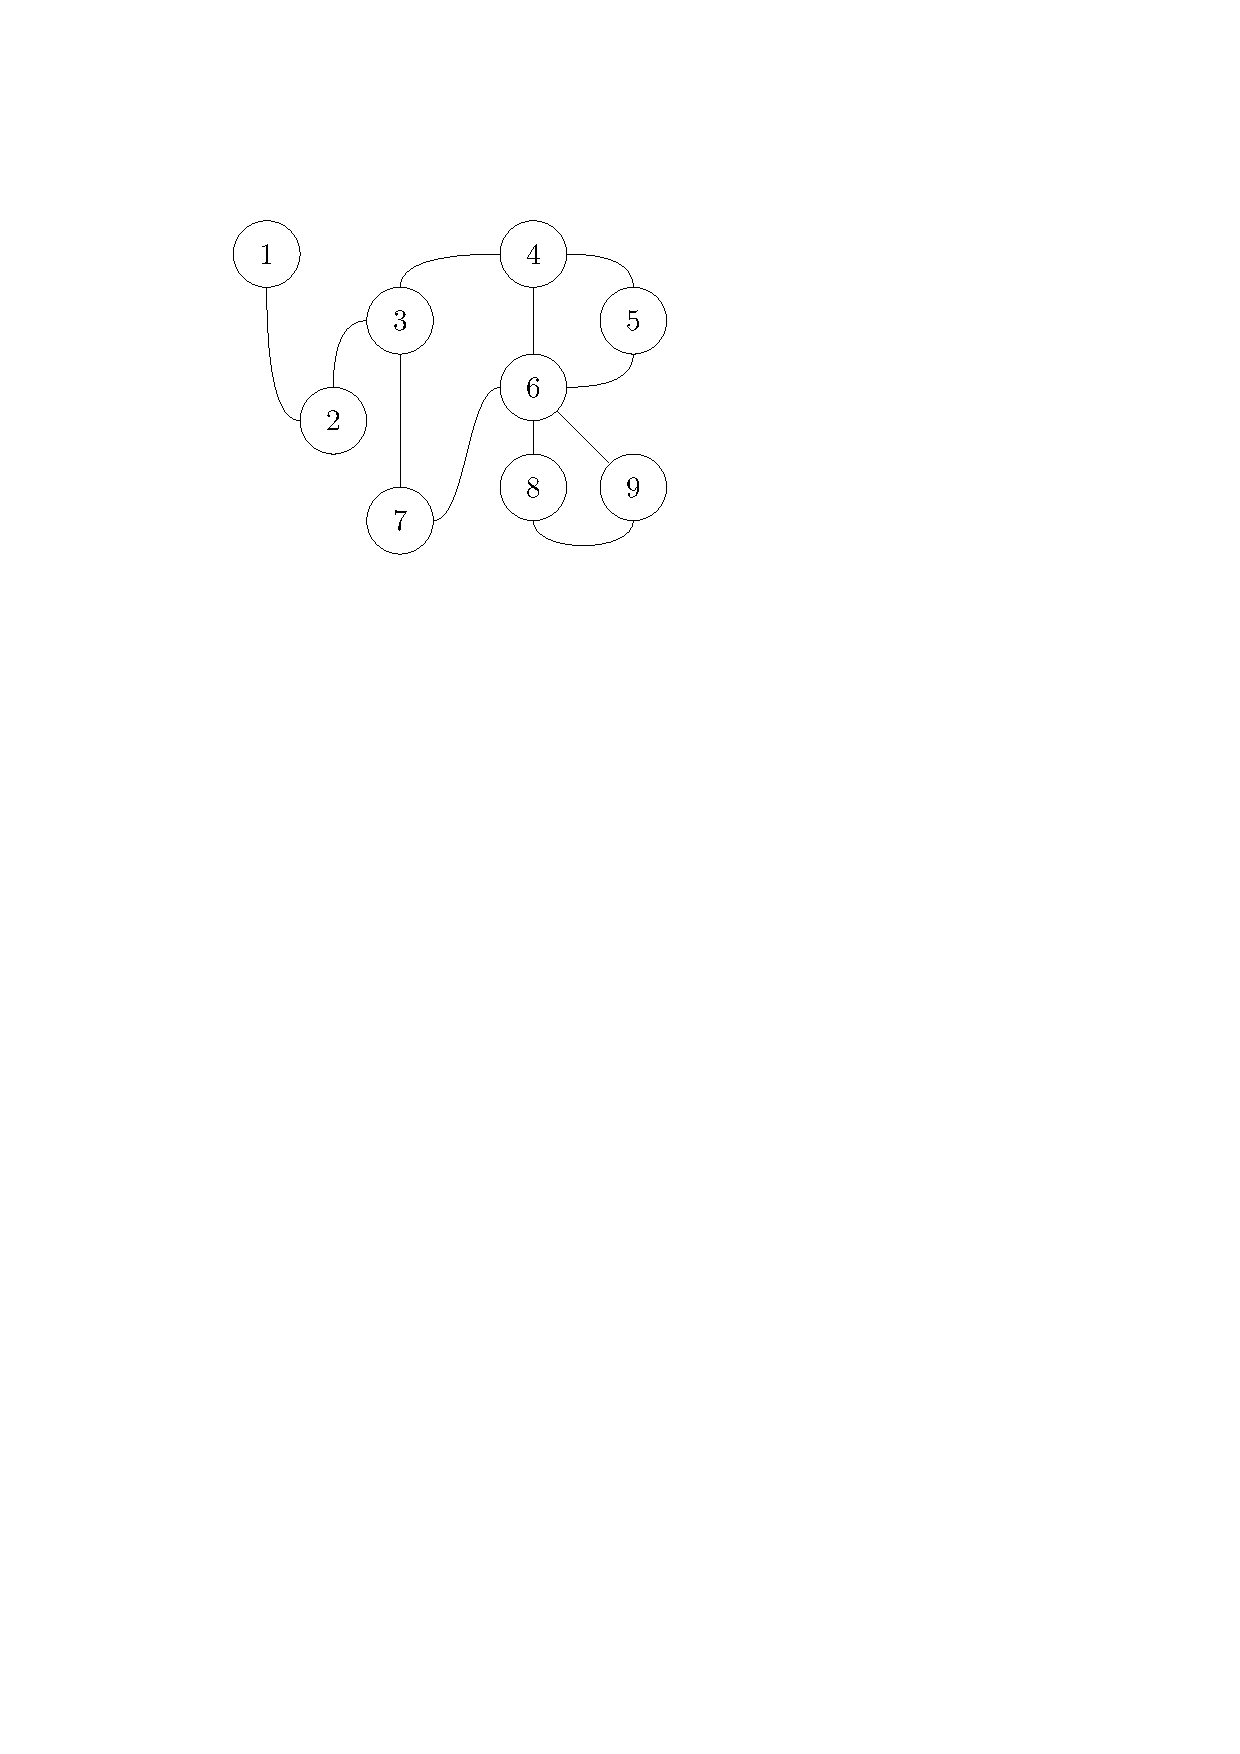
\includegraphics[width=6cm]{../../Commun/Images/python-cours-graphe-chemins-et-cycles.pdf}
\end{center}
\end{exempleUnique}

\begin{definition}
On appelle \emph{arbre} tout graphe connexe acyclique.
\end{definition}

\begin{remarques}
\remarque Les graphes suivants sont des arbres.
\begin{center}
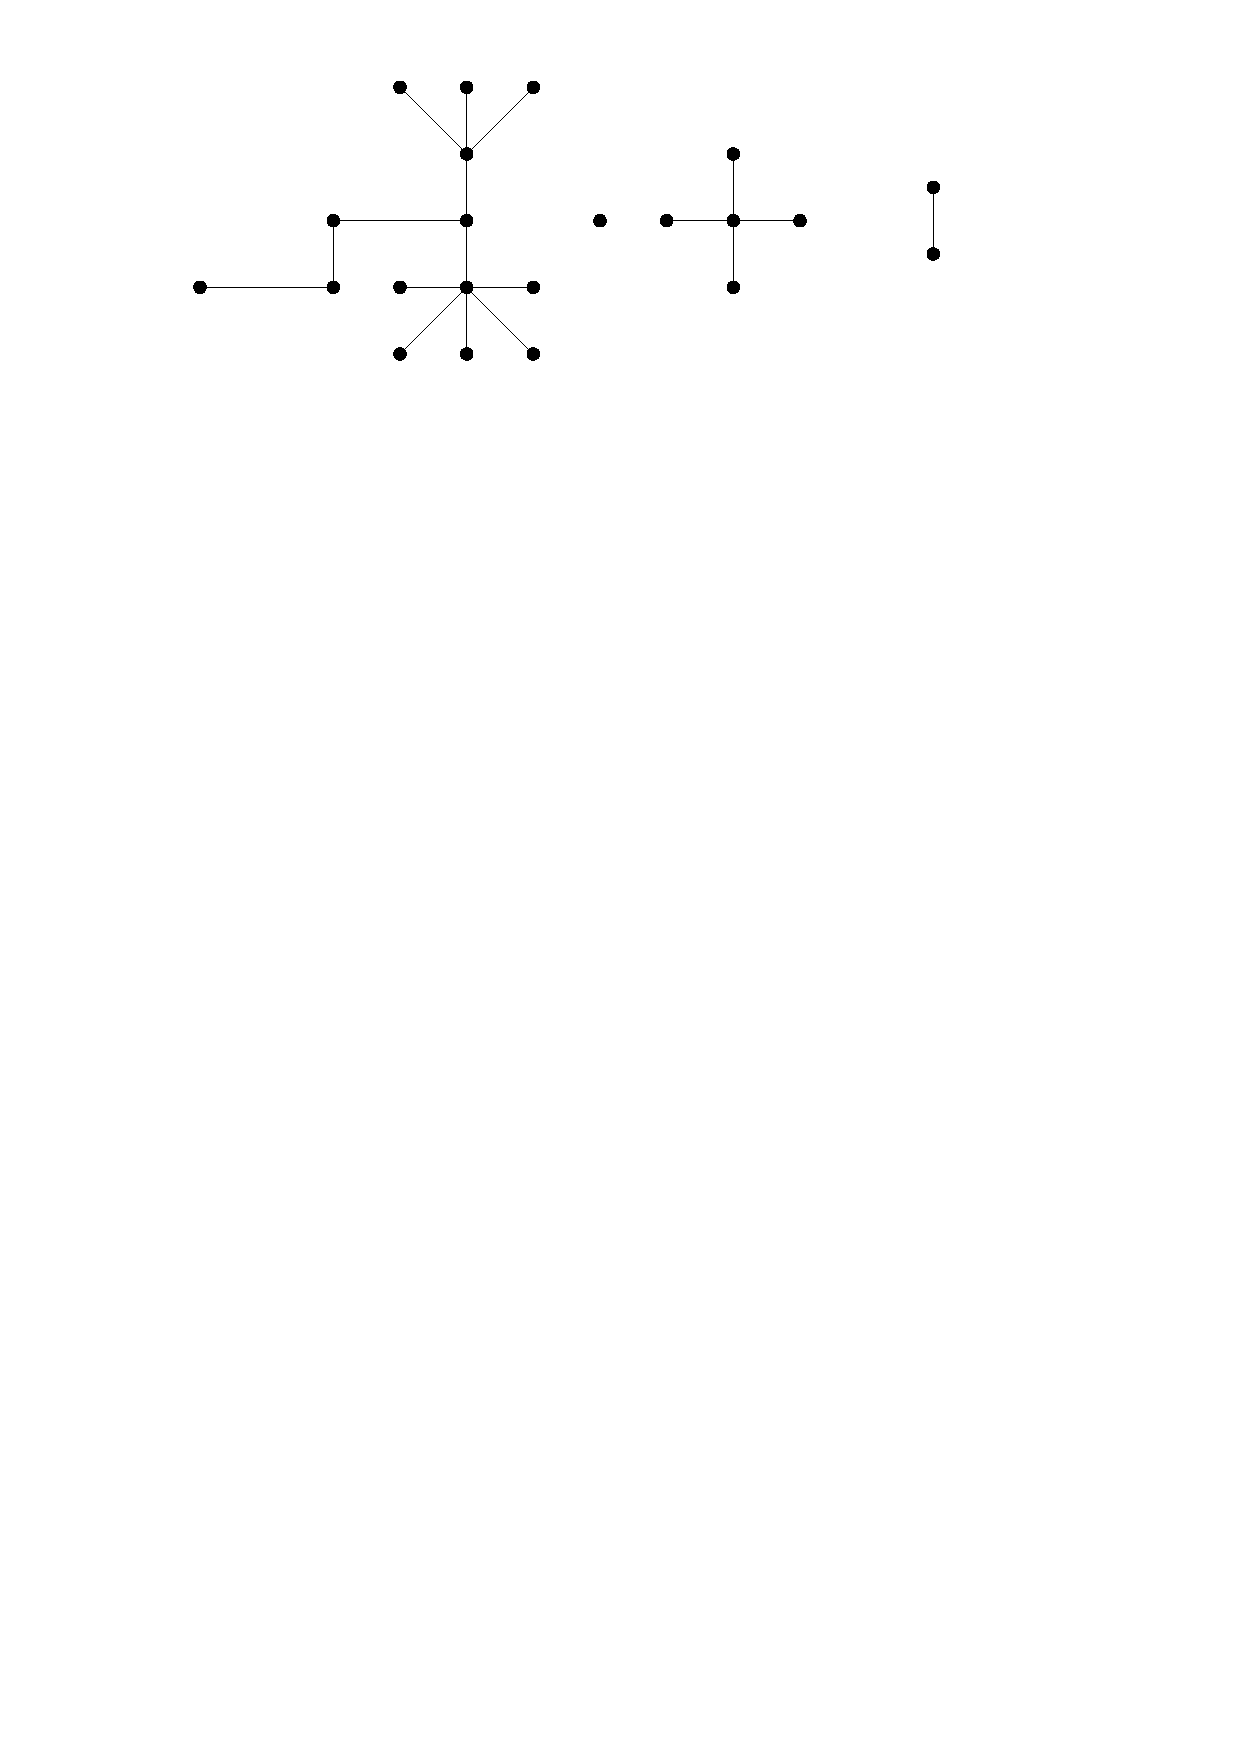
\includegraphics[width = 10cm]{../../commun/images/info-cours-graphe-theorie-foret}
\end{center}
\remarque Les arbres que nous avons manipulés dans les chapitres précédents sont ce
  qu'on appelle des \emph{arbres enracinés}. Ce sont des arbres
  pour lesquels on a choisi un sommet appelé \emph{racine}. 
  La distance d'un sommet à la racine est appelée \emph{profondeur}.
  Ces arbres sont conventionnellement dessinés de façon à ce que les sommets de même
  profondeur soient à même hauteur.
\end{remarques}
\vspace{2ex}
\begin{exoUnique}
\exo En choisissant successivement trois racines pour l'arbre de gauche ci-dessus, dessiner
  l'arbre enraciné ainsi obtenu de manière conventionnelle.
\end{exoUnique}

\subsection{Graphe orienté}

\begin{definition}
On appelle \emph{graphe orienté} tout couple $G\defeq\p{S,A}$ où
\begin{itemize}
\item $S$ est un ensemble fini non vide dont les éléments sont appelés
  \emph{sommets}.
\item $A$ est un ensemble de couples $\p{x,y}$, où $x$ et $y$ sont deux éléments
  distincts de $S$. Ces paires sont appelées \emph{arcs}.
\end{itemize}
\end{definition}
    
\begin{remarques}
\remarque En pratique, l'arc $(x,y)$ sera noté $x\to y$ ou $xy$. Intuitivement, un arc
  $x\to y$ permet de passer du sommet $x$ au sommet $y$ mais pas
  du sommet $y$ au sommet $x$. S'il y a un arc $x\to y$, on dit que $x$ est un
  \emph{prédécesseur} de $y$ et que $y$ est un \emph{successeur} de $x$.
\remarque Dans un graphe orienté
  \[\abs{A}\leq \abs{S}\p{\abs{S}-1}.\]
\remarque En pratique, on confondra souvent un graphe
  non orienté $G\defeq(S, A)$ avec son graphe orienté associé $G_{\rm o}$.
  Ce dernier possède les mêmes sommets que $G$. De plus, $x\to y$ est un arc de $G_{\rm o}$ si et
  seulement si $x-y\in A$. En particulier, dans $G_{\rm o}$,  dès que $x\to y$ est un arc,
  $y\to x$ en est un autre.
\remarque Les arbres enracinés s'orientent naturellement depuis leur racine~: lorsqu'on
  les dessine de manière conventionnelle, on les oriente du haut vers le bas. 
\remarque À un graphe orienté $G\defeq(S, A)$, on associe le graphe non orienté
  $G_{\rm no}$ obtenu en \og oubliant \fg l'orientation des arcs.
\end{remarques}
    
\begin{exemples}
\exemple Voici un exemple de graphe orienté à 7 sommets. C'est sur cet exemple que nous
  détaillerons l'exécution de nos algorithmes dans la seconde partie de ce chapitre.
\begin{center}
\begin{tikzpicture}
\node[shape=circle,draw=black,minimum size=1.2cm] (0) at (0,0) {0};
\node[shape=circle,draw=black,minimum size=1.2cm] (1) at (2,0) {1};
\node[shape=circle,draw=black,minimum size=1.2cm] (2) at (4,0) {2};
\node[shape=circle,draw=black,minimum size=1.2cm] (3) at (0,-2) {3};
\node[shape=circle,draw=black,minimum size=1.2cm] (4) at (2,-2) {4};
\node[shape=circle,draw=black,minimum size=1.2cm] (5) at (4,-2) {5};
\node[shape=circle,draw=black,minimum size=1.2cm] (6) at (6,-2) {6};
\path [-{Latex[length=3mm]}](0) edge node[left] {} (1);
\path [-{Latex[length=3mm]}](1) edge node[left] {} (2);
\path [-{Latex[length=3mm]}](0) edge node[left] {} (3);
\path [-{Latex[length=3mm]}](3) edge node[left] {} (4);
\path [-{Latex[length=3mm]}](2) edge node[left] {} (4);
\path [-{Latex[length=3mm]}](4) edge node[left] {} (1);
\path [-{Latex[length=3mm]}](2) edge node[left] {} (5);
\path [-{Latex[length=3mm]}](6) edge node[left] {} (2);
\end{tikzpicture}
\end{center}
\exemple Le graphe du web possède un sommet pour chaque page web et un arc de $x$ vers $y$
  lorsque la page $x$ contient un lien vers la page $y$. C'est ce graphe que les moteurs
  de recherche parcourent pour construire leur index. La taille du graphe du web est inconnue
  mais Google indexe plus de 50 milliards de pages.
\exemple Le graphe des utilisateurs d'Instagram a un sommet pour chaque utilisateur
  et un arc de $x$ vers $y$ lorsque $x$ est un \emph{follower} de $y$. Contrairement
  au graphe des utilisateurs de Facebook qui est non orienté, celui
  d'Instagram l'est.
\end{exemples}

\begin{definition}
Dans un graphe orienté, on appelle
\begin{itemize}
\item \emph{degré entrant} d'un sommet $x$, le nombre d'arcs de la forme $y\to x$.
\item \emph{degré sortant} d'un sommet $x$, le nombre d'arcs de la forme $x\to y$.
\item \emph{degré total} d'un sommet, la somme de son degré entrant et de son degré sortant.
\end{itemize}
\end{definition}

\begin{remarqueUnique}
\remarque Le degré entrant d'un sommet est son nombre de prédécesseurs et le
  degré sortant, son nombre de successeurs.
\end{remarqueUnique}

\begin{definition}
On appelle
chemin de longueur $n$ toute suite $c\defeq z_0,z_1,\ldots,z_{n}$ de $n+1$ sommets telle que
\[\forall k\in\interefo{0}{n}\qsep z_k \to z_{k+1}\in A.\]
Les sommets $z_0$ et $z_n$ sont appelés \emph{extrémités} du chemin et on dit que $c$
\emph{relie} $z_0$ à $z_n$. 
\end{definition}

\begin{remarques}
\remarque Comme dans les graphes non orientés, on définit la notion de chemin
  \emph{élémentaire} et de chemin \emph{simple}. Les chemins élémentaires sont simples,
  mais la réciproque est fausse.
\remarque La notion d'\emph{accessibilité} se définit aussi de la même manière. Cependant,
  dans un graphe orienté, ce n'est plus une relation d'équivalence sur $S$.
  Les notions de connexité et de composante connexe n'ont plus de sens
  pour ces graphes.
\remarque La notion de distance entre un sommet $x$ et un sommet $y$ est toujours définie. L'inégalité triangulaire reste vraie, mais
  la distance n'est plus symétrique.
\remarque La notion de cycle se définit toujours de la même manière dans un graphe
  orienté. Cependant, contrairement à ce qui se passe dans le cas des graphes non orientés,
  il existe des cycles de longueur 2.
\end{remarques}

\subsection{Graphe pondéré}

\begin{definition}
  On appelle \emph{graphe pondéré} la donnée d'un graphe
  $G\defeq\p{S,A}$ et d'une application
  $\rho:A\to\RP$ appelée \emph{poids}.
  \end{definition}



\begin{exempleUnique}
\exemple Voici le graphe non orienté des connexions ferroviaires françaises, le poids
  représentant les temps de trajet en dizaines de minutes.
\begin{center}
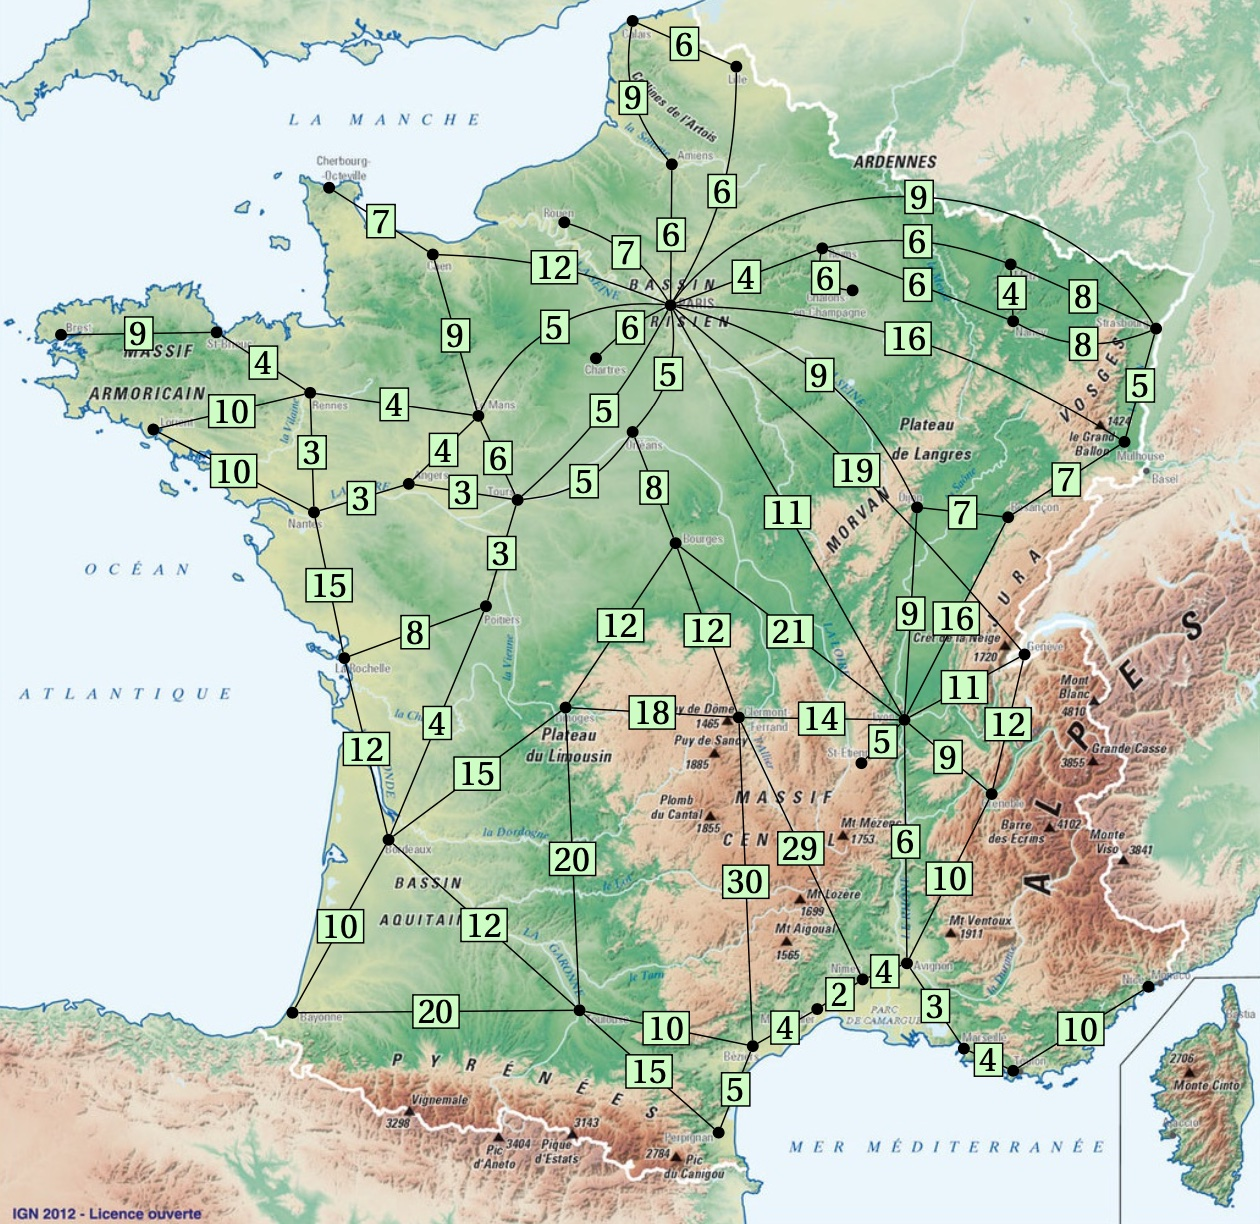
\includegraphics[width=0.5\textwidth]{../../Commun/Images/python-cours-france-train}\\
\end{center}
\end{exempleUnique}

\begin{remarques}
\remarque Un graphe pondéré peut être orienté ou non orienté.
\remarque Il est possible de considérer des graphes pondérés avec des fonctions de poids
  prenant des valeurs négatives. Mais dans ce cours, puisque c'est une condition pour
  pouvoir
  appliquer l'algorithme de Dijkstra, nous nous limiterons à des fonctions de poids
  positives.
\remarque On appelle \emph{poids du chemin} $c\defeq z_0,z_1,\ldots,z_n$ le réel
  positif
  \[\rho(c)\defeq \sum_{k=0}^{n-1} \rho(z_k z_{k+1}).\]
\remarque On appelle \emph{poids d'un graphe} la somme des poids de ses arêtes.
\end{remarques}

\begin{definition}
  Si $y$ est un sommet accessible depuis un sommet $x$, on définit
  \[\delta(x, y) \defeq \inf \ensim{\rho(c)}{c
        \textnormal{ est un chemin de } x \textnormal{ à } y}.\]
  Un \emph{chemin de poids minimal} de $x$ à $y$ est un chemin $c$
  de $x$ à $y$ tel que $\rho(c) = \delta(x, y)$.
\end{definition}

\begin{remarqueUnique}
\remarque Dans le cas où les poids sont des distances, par exemple
  si $G$ est le graphe d'un réseau routier, on pourra parler de distance et de plus court
  chemin. Il ne faut cependant pas confondre le réel $\delta(x,y)$ avec l'entier
  ${\rm d}(x,y)$ représentant le nombre minimal d'arcs entre $x$ et $y$.
\end{remarqueUnique}
  
\subsection{Représentation d'un graphe}


\begin{definition}
Soit $G\defeq\p{S,A}$ un graphe où $S=\interefo{0}{n}$. On appelle matrice d'adjacence la matrice $M\in\mat{n}{\Z}$ définie par
\[\forall i,j\in\interefo{0}{n} \qsep m_{i,j}\defeq\begin{cases}
  1 & \text{si $j$ est un successeur de  $i$,}\\
  0 & \text{sinon.}
\end{cases}\]
\end{definition}

\begin{remarques}
\remarque Un graphe est \og non orienté \fg si et seulement si sa matrice d'adjacence est symétrique.
\remarque Puisqu'on interdit les boucles, une matrice d'adjacence n'a
  que des 0 sur la diagonale.
\remarque On peut représenter un graphe pondéré par une matrice d'adjacence $M\in\mat{n}{\R}$. On prend
    pour coefficient $m_{i,j}$ la valeur \verb!None! lorsqu'il n'existe pas d'arc
    de $i$ à $j$, et le poids $\rho_{i,j}$ de l'arc allant de $i$ à $j$
    lorsqu'un tel arc existe. 
\end{remarques}

\begin{definition}
Soit $G\defeq\p{S,A}$ un graphe où $S=\interefo{0}{n}$. On appelle liste d'adjacence le tableau $g$ de longueur
$n$ tel que
pour tout $i\in\interefo{0}{n}$, $g_i$ est la liste des successeurs $j\in\interefo{0}{n}$
de $i$.
\end{definition}

\begin{remarqueUnique}
\remarque On peut représenter un graphe pondéré par une liste d'adjacence
    dans laquelle, pour tout sommet $i$, $g_i$ est la liste des couples
    $(\rho_{i,j},j)$ où $j$ est un successeur de $i$.
\remarque Dans la suite de ce
    cours, nous utiliserons des listes d'adjacence pour stocker les graphes pondérés.
\end{remarqueUnique}


\section{Algorithmes sur les graphes}

\subsection{Parcours générique d'un graphe}

Supposons que vous êtes enfermé dans un labyrinthe de salles, connectées entre elles
par des portes. Nous représentons ce labyrinthe par un graphe dont les sommets sont
les salles et les arêtes sont les portes reliant ces salles entre elles. Si l'on souhaite sortir de ce labyrinthe,
un réflexe naturel est d'emprunter au hasard les portes que l'on croise. Cependant,
cette stratégie possède deux défauts importants~: elle ne nous dit pas ce qu'on doit
faire lorsqu'on tombe dans un cul-de-sac et elle ne nous empêche pas de tourner en rond.\\

Pour résoudre ces deux problèmes, la solution la plus simple est de marquer les
salles. Au cours de notre exploration, nous choisirons donc de les placer
successivement dans 3 états différents~:
\begin{itemize}
\item \emph{Inconnu}~: C'est l'état dans lequel est une salle qui n'a pas encore été
  découverte.
\item \emph{Découvert}~: C'est l'état dans lequel on place une salle lorsqu'on l'a aperçue
  par une porte.
\item \emph{Visité}~: C'est l'état dans lequel est une salle dans laquelle nous sommes
  déjà entrés.
\end{itemize}
Pour ne pas tourner en rond, il suffit de ne pas entrer dans une salle qui a déjà
été visitée. Pour ces salles, on peut choisir de marquer leur sol d'une croix blanche.
Et pour savoir que faire lorsqu'on est dans un cul-de-sac, il suffit de garder une trace
des salles que l'on a découvertes, mais qui n'ont pas encore été visitées. Pour cela, on
conserve avec nous un sac contenant une marque pour chacune d'elles.\\

Revenons au vocabulaire des graphes. À l'aide de ces deux outils, notre sac ainsi que le
marquage des sommets, nous sommes armés pour parcourir l'ensemble des sommets accessibles
depuis notre sommet de départ. Ce sommet est appelé \emph{source}. Pour cela, il
nous suffit de suivre
l'algorithme suivant, que nous appelons \og \emph{parcours générique} \fg.
% \begin{center}
% \begin{minipage}{0.5\linewidth}
% \begin{algorithm}[H]
% \caption{Parcours générique}
% \begin{algorithmic}
% \State mettre le sommet \emph{source} dans le \emph{sac}
% \While{le \emph{sac} n'est pas vide}
%   \State prendre un sommet $x$ dans le $sac$
%   \If{$x$ n'a pas été visité}
%     \State marquer le sommet $x$ comme visité
%     \For{chaque arc $xy$}
%       \State mettre le sommet $y$ dans le sac
%     \EndFor 
%   \EndIf
% \EndWhile
% \end{algorithmic}
% \end{algorithm}
% \end{minipage}
% \end{center}
\begin{center}
  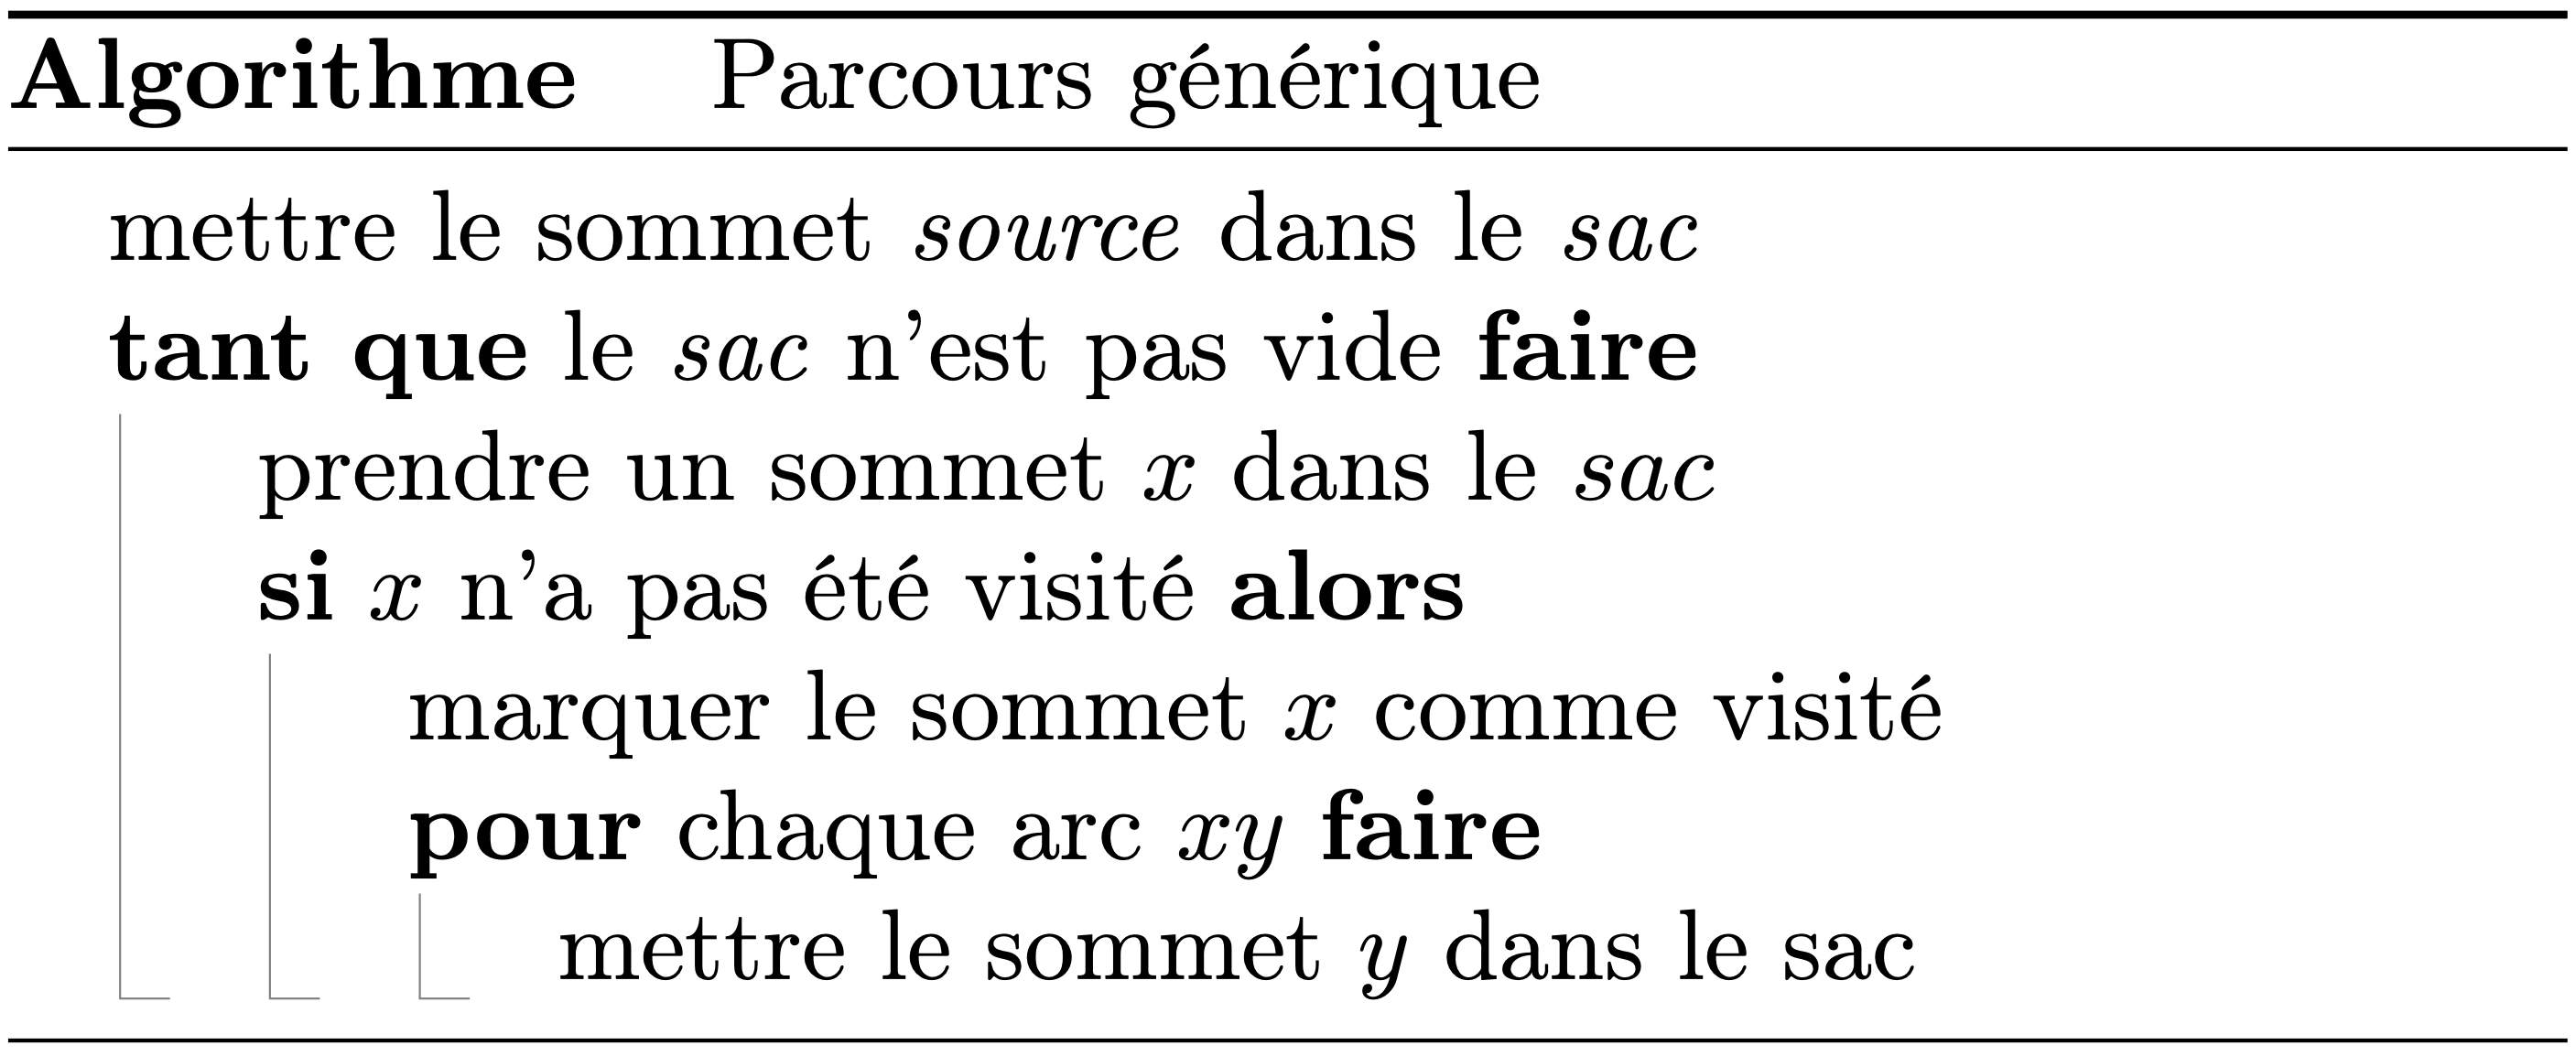
\includegraphics[width=0.5\textwidth]{../../Commun/Images/python-cours-parcours_generique}
\end{center}
\vspace{2ex}
\noindent
La seule propriété dont notre sac a besoin est qu'on puisse y mettre des
sommets pour les extraire plus tard. L'ordre dans lesquels ces sommets sont extraits
n'a pas d'importance pour le moment.

\begin{proposition}
L'algorithme de parcours générique visite tous les sommets accessibles depuis la source
et uniquement ceux-là.
\end{proposition}

Supposons que l'on garde en mémoire le sommet depuis lequel on visite chaque sommet,
en ne mettant pas le sommet $y$ dans notre sac, mais plutôt le couple $(x, y)$.
Un parcours
générique mettra ainsi en valeur un arbre, enraciné en la source, couvrant l'ensemble des
sommets accessibles. Par exemple, en considérant
le graphe ci-dessous,

\begin{center}
\begin{tikzpicture}
\node[shape=circle,draw=black,minimum size=1.2cm] (0) at (0,0) {0};
\node[shape=circle,draw=black,minimum size=1.2cm] (1) at (2,0) {1};
\node[shape=circle,draw=black,minimum size=1.2cm] (2) at (4,0) {2};
\node[shape=circle,draw=black,minimum size=1.2cm] (3) at (0,-2) {3};
\node[shape=circle,draw=black,minimum size=1.2cm] (4) at (2,-2) {4};
\node[shape=circle,draw=black,minimum size=1.2cm] (5) at (4,-2) {5};
\node[shape=circle,draw=black,minimum size=1.2cm] (6) at (6,-2) {6};
\path [-{Latex[length=3mm]}](0) edge node[left] {} (1);
\path [-{Latex[length=3mm]}](1) edge node[left] {} (2);
\path [-{Latex[length=3mm]}](0) edge node[left] {} (3);
\path [-{Latex[length=3mm]}](3) edge node[left] {} (4);
\path [-{Latex[length=3mm]}](2) edge node[left] {} (4);
\path [-{Latex[length=3mm]}](4) edge node[left] {} (1);
\path [-{Latex[length=3mm]}](2) edge node[left] {} (5);
\path [-{Latex[length=3mm]}](6) edge node[left] {} (2);
\end{tikzpicture}
\end{center}

\noindent
si les couples que l'on sort du sac sont successivement $(\emptyset,0)$, $(0, 1)$,
$(1, 2)$, $(0,3)$, $(2,4)$ et $(2,5)$, on obtient l'arbre enraciné suivant~:

\begin{center}
\begin{tikzpicture}
\node[shape=circle,fill=colorLazoBlue1Light,draw=black,minimum size=1.2cm] (0) at (0,0) {0};
\node[shape=circle,fill=colorLazoBlue1Light,draw=black,minimum size=1.2cm] (1) at (2,0) {1};
\node[shape=circle,fill=colorLazoBlue1Light,draw=black,minimum size=1.2cm] (2) at (4,0) {2};
\node[shape=circle,fill=colorLazoBlue1Light,draw=black,minimum size=1.2cm] (3) at (0,-2) {3};
\node[shape=circle,fill=colorLazoBlue1Light,draw=black,minimum size=1.2cm] (4) at (2,-2) {4};
\node[shape=circle,fill=colorLazoBlue1Light,draw=black,minimum size=1.2cm] (5) at (4,-2) {5};
\node[shape=circle,draw=black,minimum size=1.2cm] (6) at (6,-2) {6};
\path [-{Latex[length=3mm,color=colorLazoPink1]},draw=colorLazoPink1](0) edge node[left] {} (1);
\path [-{Latex[length=3mm,color=colorLazoPink1]},draw=colorLazoPink1](1) edge node[left] {} (2);
\path [-{Latex[length=3mm,color=colorLazoPink1]},draw=colorLazoPink1](0) edge node[left] {} (3);
\path [-{Latex[length=3mm,color=black!30]},draw=black!30](3) edge node[left] {} (4);
\path [-{Latex[length=3mm,color=colorLazoPink1]},draw=colorLazoPink1](2) edge node[left] {} (4);
\path [-{Latex[length=3mm,color=black!30]},draw=black!30](4) edge node[left] {} (1);
\path [-{Latex[length=3mm,color=colorLazoPink1]},draw=colorLazoPink1](2) edge node[left] {} (5);
\path [-{Latex[length=3mm,color=black!30]},draw=black!30](6) edge node[left] {} (2);
\end{tikzpicture}
\end{center}
\noindent
Par la suite, nous utiliserons principalement nos sacs pour y placer des sommets.
Cependant, lors de certains raisonnements, il sera parfois utile de faire comme si on y
avait placé un couple.\\

La structure de données que nous allons utiliser pour implémenter notre sac va déterminer
l'ordre dans lequel les sommets en sont extraits.
\begin{itemize}
\item \emph{Pile}~: Si nous utilisons une pile, pour laquelle c'est le dernier sommet qui
  a été placé dans le sac qui en est extrait, nous obtiendrons ce qu'on appelle
  un \emph{parcours en profondeur}. Bien que tous les parcours nous permettent
  d'obtenir l'ensemble des sommets accessibles depuis un sommet, la simplicité de la
  structure de pile fait que c'est souvent ce parcours que nous utiliserons pour cela.
  Nous verrons aussi que le parcours en profondeur nous permet de détecter les cycles
  dans un graphe.
\item \emph{File}~: Si nous utilisons une file, pour laquelle c'est le premier sommet
  qui a été placé dans le sac qui en est extrait, nous obtiendrons ce qu'on appelle
  un \emph{parcours en largeur}. Ce parcours nous sera utile pour trouver le chemin
  de longueur minimale entre la source et les sommets accessibles depuis cette
  dernière.
\item \emph{File de priorité}~: L'utilisation d'une file de priorité nous permettra
  de découvrir une famille d'algorithmes fonctionnant avec les graphes pondérés. Ils
  se distinguent par les différentes priorités qu'ils utilisent.
  \begin{itemize}
  \item \emph{Dijkstra}~: L'algorithme de Dijkstra nous permet de trouver le chemin
    de poids minimal entre la source et les sommets accessibles depuis cette dernière.
    Pour cela, la
    priorité utilisée est le poids du chemin qui nous a permis de découvrir le sommet.
  \item \emph{Prim}~: L'algorithme de Prim nous permet de trouver un arbre de poids minimal
    couvrant l'ensemble des sommets accessibles. Pour cela, la priorité que nous utiliserons est
    le poids de l'arc qui nous a permis de découvrir le sommet.
  \end{itemize}
\end{itemize}

\vspace{2ex}
Commençons par étudier le plus simple de ces parcours~: le parcours en profondeur.

\subsection{Parcours en profondeur}

\subsubsection{Version itérative}

L'implémentation Python du parcours en profondeur se fait naturellement. On suppose
ici que $\mathcal{S}\defeq\interefo{0}{n}$ et que le graphe est représenté par sa liste
d'adjacence. Pour marquer les sommets, nous utilisons le tableau \emph{visité}, de
longueur $n$, dont tous les éléments sont initialisés à \verb!False!. Pour le sac,
nous utilisons la liste \emph{pile} que nous utilisons, comme son nom l'indique, comme
une pile.

\begin{pythoncodeline}
def profondeur(g, s):
    """profondeur(g: list[list[int]], s: int) -> NoneType"""
    n = len(g)
    visite = [False for _ in range(n)]
    pile = [s]
    while len(pile) != 0:
        x = pile.pop()
        if not visite[x]:
            visite[x] = True
            for y in g[x]:
                pile.append(y)
\end{pythoncodeline}
\noindent
Si l'on souhaite effectuer une action pour chaque
sommet, il suffit de définir une fonction \verb!f(x: int) -> NoneType! que l'on appelle
juste avant l'instruction \verb!visite[x] = True!. Par exemple, si l'on souhaite afficher
à l'écran les sommets visités dans l'ordre de notre parcours, il suffit d'insérer \verb!print(x)! ligne 9.

\begin{center}
\begin{tikzpicture}
\node[shape=circle,draw=black,minimum size=1.2cm] (0) at (0,0) {0};
\node[shape=circle,draw=black,minimum size=1.2cm] (1) at (2,0) {1};
\node[shape=circle,draw=black,minimum size=1.2cm] (2) at (4,0) {2};
\node[shape=circle,draw=black,minimum size=1.2cm] (3) at (0,-2) {3};
\node[shape=circle,draw=black,minimum size=1.2cm] (4) at (2,-2) {4};
\node[shape=circle,draw=black,minimum size=1.2cm] (5) at (4,-2) {5};
\node[shape=circle,draw=black,minimum size=1.2cm] (6) at (6,-2) {6};
\path [-{Latex[length=3mm]}](0) edge node[left] {} (1);
\path [-{Latex[length=3mm]}](1) edge node[left] {} (2);
\path [-{Latex[length=3mm]}](0) edge node[left] {} (3);
\path [-{Latex[length=3mm]}](3) edge node[left] {} (4);
\path [-{Latex[length=3mm]}](2) edge node[left] {} (4);
\path [-{Latex[length=3mm]}](4) edge node[left] {} (1);
\path [-{Latex[length=3mm]}](2) edge node[left] {} (5);
\path [-{Latex[length=3mm]}](6) edge node[left] {} (2);
\end{tikzpicture}
\end{center}

Illustrons son fonctionnement en détail sur un exemple. Le tableau ci-dessous détaille
les différentes étapes du parcours en profondeur du présent graphe à partir du sommet 0.
Le contenu de la \emph{pile} est détaillé lors du passage ligne 6, tout comme
l'ensemble des sommets marqués dans \emph{visité}.

\begin{center}
\begin{tabular}{l|l|l}
\emph{pile} & \emph{visité} & action\\
\hline
\verb_[0]_ & $\ens{}$  & Dépiler 0, le marquer et empiler ses successeurs 1 et 3.\\
\verb_[1, 3]_ & $\ens{0}$ & Dépiler 3, le marquer et empiler son successeur 4.\\
\verb_[1, 4]_ & $\ens{0, 3}$ & Dépiler 4, le marquer et empiler son successeur 1.\\
\verb_[1, 1]_ & $\ens{0, 3, 4}$ & Dépiler 1, le marquer et empiler son successeur 2.\\
\verb_[1, 2]_ & $\ens{0, 1, 3, 4}$ & Dépiler 2, le marquer et empiler ses successeurs 4 et 5.\\
\verb_[1, 4, 5]_ & $\ens{0, 1, 2, 3, 4}$ & Dépiler 5 et le marquer. Il n'a pas de successeur.\\
\verb_[1, 4]_ & $\ens{0, 1, 2, 3, 4, 5}$ & Dépiler 4. Il a déjà été marqué.\\
\verb_[1]_ & $\ens{0, 1, 2, 3, 4, 5}$ & Dépiler 1. Il a déjà été marqué.\\
\verb_[]_ & $\ens{0, 1, 2, 3, 4, 5}$ & \emph{pile} est vide donc l'algorithme se termine.
\end{tabular}
\end{center}
Une fois le parcours terminé, tous les sommets atteignables à partir du sommet 0 ont été
marqués, à savoir $0, 1, 2, 3, 4$ et 5. Inversement, le sommet 6, qui n'est pas atteignable
à partir de 0 n'a pas été marqué. C'est là une propriété fondamentale du parcours en
profondeur. Le graphe ci-dessous met en valeur les sommets visités ainsi que les
arcs empruntés lors de ce parcours.

\begin{center}
\begin{tikzpicture}
\node[shape=circle,fill=colorLazoBlue1Light,draw=black,minimum size=1.2cm] (0) at (0,0) {0};
\node[shape=circle,fill=colorLazoBlue1Light,draw=black,minimum size=1.2cm] (1) at (2,0) {1};
\node[shape=circle,fill=colorLazoBlue1Light,draw=black,minimum size=1.2cm] (2) at (4,0) {2};
\node[shape=circle,fill=colorLazoBlue1Light,draw=black,minimum size=1.2cm] (3) at (0,-2) {3};
\node[shape=circle,fill=colorLazoBlue1Light,draw=black,minimum size=1.2cm] (4) at (2,-2) {4};
\node[shape=circle,fill=colorLazoBlue1Light,draw=black,minimum size=1.2cm] (5) at (4,-2) {5};
\node[shape=circle,draw=black,minimum size=1.2cm] (6) at (6,-2) {6};
\path [-{Latex[length=3mm,color=black!30]},draw=black!30](0) edge node[left] {} (1);
\path [-{Latex[length=3mm,color=colorLazoPink1]},draw=colorLazoPink1](1) edge node[left] {} (2);
\path [-{Latex[length=3mm,color=colorLazoPink1]},draw=colorLazoPink1](0) edge node[left] {} (3);
\path [-{Latex[length=3mm,color=colorLazoPink1]},draw=colorLazoPink1](3) edge node[left] {} (4);
\path [-{Latex[length=3mm,color=black!30]},draw=black!30](2) edge node[left] {} (4);
\path [-{Latex[length=3mm,color=colorLazoPink1]},draw=colorLazoPink1](4) edge node[left] {} (1);
\path [-{Latex[length=3mm,color=colorLazoPink1]},draw=colorLazoPink1](2) edge node[left] {} (5);
\path [-{Latex[length=3mm,color=black!30]},draw=black!30](6) edge node[left] {} (2);
\end{tikzpicture}
\end{center}

\subsubsection{Version récursive}

Le parcours en profondeur est un algorithme fondamentalement récursif dont voici une
implémentation Python~:

\begin{pythoncodeline}
def profondeur_rec(g, visite, x):
    """profondeur_rec(g: list[list[int]], visite: list[bool],
                      x: int) -> NoneType"""
    if not visite[x]:
        visite[x] = True
        for y in g[x]:
            profondeur_rec(g, visite, y)
\end{pythoncodeline}
\noindent
Pour lancer un parcours en profondeur depuis un sommet $s$, on utilisera la fonction
suivante~:
\begin{pythoncodeline}
def profondeur(g, s):
    """profondeur(g: list[list[int]], s: int) -> NoneType"""
    n = len(g)
    visite = [False for _ in range(n)]
    profondeur_rec(g, visite, s)
\end{pythoncodeline}
\noindent
Dans cette version, une pile est toujours présente par l'intermédiaire de la pile d'appels.
Contrairement à ce qui se passe dans la version itérative, les sommets sont visités dès
qu'ils sont découverts; en récursif, ces deux états sont donc confondus.
Le tableau ci-dessous détaille l'ensemble des sommets marqués dans \emph{visité} au
moment de l'appel de \verb!profondeur_rec!.
La pile d'appel est aussi représentée dans la colonne \og chemin emprunté \fg.


\begin{center}
\begin{tabular}{l|l|l}
\emph{visité} & chemin emprunté & action\\
\hline
$\ens{}$ &0 &  Marquer 0, emprunter l'arc $0\to 1$.\\
$\ens{0}$ &$0 \to 1$ & Marquer 1, emprunter l'arc $1\to 2$.\\ 
$\ens{0,1}$ &$0 \to 1 \to 2$ & Marquer 2, emprunter l'arc $2\to 4$.\\
$\ens{0, 1, 2}$ &$0 \to 1 \to 2 \to 4$ & Marquer 4, emprunter l'arc $4\to 1$.\\
$\ens{0, 1, 2, 4}$ &$0 \to 1 \to 2 \to 4 \to 1$ & Déjà découvert.\\
$\ens{0,1,2,4}$ &$0 \to 1 \to 2 \to 4$ & Pas d'autre arc, terminé.\\
$\ens{0,1,2,4}$ &$0 \to 1 \to 2$ & Emprunter l'arc $2\to 5$.\\
$\ens{0,1,2,4,5}$ &$0 \to 1 \to 2 \to 5$ & Marquer 5, aucun arc, terminé.\\
$\ens{0,1,2,4,5}$ &$0 \to 1 \to 2$ & Pas d'autre arc, terminé.\\
$\ens{0,1,2,4,5}$ &$0 \to 1$ & Pas d'autre arc, terminé.\\
$\ens{0,1,2,4,5}$ &$0$ & Emprunter l'arc $0\to 3$.\\ 
$\ens{0,1,2,4,5}$ &$0 \to 3$ & Marquer 3, emprunter l'arc $3\to 4$.\\
$\ens{0,1,2,3,4,5}$ & $0 \to 3 \to 4$ & Déjà découvert.\\
$\ens{0,1,2,3,4,5}$ & $0 \to 3$ & Pas d'autre arc, terminé.\\
$\ens{0,1,2,3,4,5}$ & $0$ & Pas d'autre arc, terminé.
\end{tabular}
\end{center}
\noindent
\noindent
On remarque que même si les sommets visités sont les mêmes que dans la version itérative,
les arcs empruntés diffèrent~: le parcours que l'on vient
d'effectuer est un autre parcours en profondeur.


\begin{center}
\begin{tikzpicture}
\node[shape=circle,fill=colorLazoBlue1Light,draw=black,minimum size=1.2cm] (0) at (0,0) {0};
\node[shape=circle,fill=colorLazoBlue1Light,draw=black,minimum size=1.2cm] (1) at (2,0) {1};
\node[shape=circle,fill=colorLazoBlue1Light,draw=black,minimum size=1.2cm] (2) at (4,0) {2};
\node[shape=circle,fill=colorLazoBlue1Light,draw=black,minimum size=1.2cm] (3) at (0,-2) {3};
\node[shape=circle,fill=colorLazoBlue1Light,draw=black,minimum size=1.2cm] (4) at (2,-2) {4};
\node[shape=circle,fill=colorLazoBlue1Light,draw=black,minimum size=1.2cm] (5) at (4,-2) {5};
\node[shape=circle,draw=black,minimum size=1.2cm] (6) at (6,-2) {6};
\path [-{Latex[length=3mm,color=colorLazoPink1]},draw=colorLazoPink1](0) edge node[left] {} (1);
\path [-{Latex[length=3mm,color=colorLazoPink1]},draw=colorLazoPink1](1) edge node[left] {} (2);
\path [-{Latex[length=3mm,color=colorLazoPink1]},draw=colorLazoPink1](0) edge node[left] {} (3);
\path [-{Latex[length=3mm,color=black!30]},draw=black!30](3) edge node[left] {} (4);
\path [-{Latex[length=3mm,color=colorLazoPink1]},draw=colorLazoPink1](2) edge node[left] {} (4);
\path [-{Latex[length=3mm,color=black!30]},draw=black!30](4) edge node[left] {} (1);
\path [-{Latex[length=3mm,color=colorLazoPink1]},draw=colorLazoPink1](2) edge node[left] {} (5);
\path [-{Latex[length=3mm,color=black!30]},draw=black!30](6) edge node[left] {} (2);
\end{tikzpicture}
\end{center}

\subsubsection{Accessibilité, connexité}

Une application immédiate du parcours en profondeur consiste à déterminer s'il existe un
chemin entre deux sommets $x$ et $y$. Pour cela, il suffit de lancer un parcours
en profondeur à partir du sommet $x$ puis, une fois qu'il est terminé, de regarder si le
sommet $y$ fait partie des sommets visités. Le programme suivant
réalise cet algorithme~:

\begin{pythoncodeline}
def existe_chemin(g, x, y):
    """existe_chemin(g: list[list[int]], x: int, y: int) -> bool""" 
    n = len(g)
    visite = [False for _ in range(n)]
    profondeur_rec(g, visite, x)
    return visite[y]
\end{pythoncodeline}

\noindent
Le parcours en profondeur 
est un algorithme très efficace, dont la complexité
temporelle est de l'ordre du nombre de sommets du graphe (pour l'initialisation de \emph{visité})
auquel on ajoute le nombre d'arcs qui sont examinés pendant ce parcours. On a donc une
complexité temporelle 
en ${\rm O}(\abs{S}+\abs{A})$. En effet, chaque arc
$x\to y$ est examiné au plus une fois, à savoir la première fois que la fonction
\verb!profondeur_rec! est appelée sur le sommet $x$~: si la fonction
\verb!profondeur_rec! est rappelée plus tard sur ce même sommet $x$, alors il
sera trouvé dans \emph{visité} et la fonction se terminera immédiatement. Dans le pire des cas, tous les sommets sont atteignables et le graphe
est entièrement parcouru. Le cout est moindre lorsque certains sommets ne sont pas atteignables
depuis le sommet de départ.\\

La complexité spatiale de la version récursive est en $\Theta(\abs{S})$~: cette
complexité provient du tableau \emph{visité} dont
la taille est $\abs{S}$, auquel on ajoute la taille de la pile
d'appels qui reste toujours inférieure au nombre de sommets puisque la succession de
sommets passés en argument des appels actifs forme à
chaque instant un chemin élémentaire.\\

On peut aussi tester la connexité d'un graphe non orienté de la même manière. On utilise pour
cela la fonction \verb!est_connexe!~:
\begin{pythoncodeline}
def tous_vrai(t):
    """tous_vrai(t: list[bool]) -> bool"""
    for v in t:
        if not v:
            return False
    return True

def est_connexe(g):
    """est_connexe(g: list[list[int]]) -> bool"""
    n = len(g)
    visite = [False for _ in range(n)]
    profondeur_rec(g, visite, 0)
    return tous_vrai(visite)
\end{pythoncodeline}
\noindent
Cet algorithme a de nouveau une complexité temporelle en ${\rm O}(\abs{S}+\abs{A})$ et
une complexité spatiale en $\Theta(\abs{S})$.

\begin{exoUnique}
\exo Écrire une fonction qui compte le nombre de composantes connexes d'un graphe non
  orienté.
\end{exoUnique}

\subsubsection{Détection de cycle}

Le parcours en profondeur permet également de détecter la présence d'un cycle dans un
graphe orienté. En effet, puisque l'on marque les sommets avant de considérer leurs voisins,
pour justement éviter de tourner en rond dans un cycle, alors on doit pouvoir être à même
de détecter leur présence. Il y a cependant une subtilité, car lorsqu'on retombe
sur un sommet déjà marqué, on ne sait pas pour autant si l'on vient de découvrir un cycle.
Considérons par exemple le parcours en profondeur des deux graphes suivants, à partir
du sommet 0 à chaque fois.

\begin{center}
\begin{tikzpicture}
\node[shape=circle,draw=black,minimum size=1.2cm] (0) at (0,0) {0};
\node[shape=circle,draw=black,minimum size=1.2cm] (1) at (2,2) {1};
\node[shape=circle,draw=black,minimum size=1.2cm] (2) at (4,0) {2};
\node[shape=circle,draw=black,minimum size=1.2cm] (3) at (2,-2) {3};
\path [-{Latex[length=3mm]}](0) edge node[left] {} (1);
\path [-{Latex[length=3mm]}](1) edge node[left] {} (2);
\path [-{Latex[length=3mm]}](0) edge node[left] {} (3);
\path [-{Latex[length=3mm]}](3) edge node[left] {} (2);
\end{tikzpicture}
\hspace{2cm}
\begin{tikzpicture}
\node[shape=circle,draw=black,minimum size=1.2cm] (0) at (0,0) {0};
\node[shape=circle,draw=black,minimum size=1.2cm] (1) at (2,2) {1};
\node[shape=circle,draw=black,minimum size=1.2cm] (2) at (4,0) {2};
\node[shape=circle,draw=black,minimum size=1.2cm] (3) at (2,-2) {3};
\path [-{Latex[length=3mm]}](0) edge node[left] {} (1);
\path [-{Latex[length=3mm]}](1) edge node[left] {} (2);
\path [-{Latex[length=3mm]}](3) edge node[left] {} (1);
\path [-{Latex[length=3mm]}](2) edge node[left] {} (3);
\end{tikzpicture}
\end{center}
\noindent
Dans le graphe de gauche, on retombe sur le sommet 2. Il n'y a pas de cycle pour autant,
mais seulement un chemin parallèle. Dans le graphe de droite, on retombe sur
le sommet 1, cette fois à cause d'un cycle. Tel qu'il est écrit, notre parcours en
profondeur ne nous permet pas de distinguer ces deux situations. Dans les deux cas, 
on constate que le sommet est déjà visité sans pouvoir en tirer de conclusion quant à
l'existence d'un cycle.\\

Pour y remédier, on va distinguer dans notre marquage trois sortes de sommets~:
ceux que l'on n'a pas encore découverts qui seront marqués comme \emph{inconnu}, ceux que
l'on a \emph{découvert} mais qui sont toujours présents dans le chemin déterminé
par la pile d'appels (ces sommets sont donc \emph{visités} puisque nous
utilisons une implémentation récursive dans laquelle ces deux états sont confondus),
et ceux qui ne sont plus présents dans la pile d'appels,
qu'on marquera comme \emph{fermé}.
Le parcours en profondeur est modifié de la manière suivante~: lorsqu'on visite un sommet
$x$
\begin{itemize}
\item S'il est marqué comme \og découvert \fg, c'est qu'on vient de découvrir un cycle.
\item S'il est marqué comme \og fermé \fg, on ne fait rien.
\item S'il est marqué comme \og inconnu \fg, on procède ainsi~:
  \begin{itemize}
  \item On marque le sommet $x$ comme \og découvert \fg.
  \item On visite tous ses successeurs, récursivement.
  \item Enfin, on le marque comme \og fermé \fg.
  \end{itemize}
\end{itemize}
Comme on le voit, les successeurs du sommet $x$ sont examinés après le moment où $x$
est marqué comme \og découvert \fg et avant le moment où il est marqué comme
\og fermé \fg. Ainsi, s'il existe un cycle nous ramenant sur $x$, on le trouvera
comme étant \og découvert \fg et le cycle sera signalé.\\

Le programme suivant réalise cette détection de cycle.
La fonction \verb!possede_cycle_rec(g, x, etat)! est toujours une fonction récursive, mais
elle renvoie désormais un résultat, à savoir un booléen indiquant la présence d'un cycle.
Enfin, la fonction \verb!possede_cycle! marque tous les sommets comme \og inconnu \fg puis
lance un parcours
en profondeur à partir de tous les sommets du graphe. Si l'un de ces parcours renvoie
\verb!True!, on transmet ce résultat. Sinon, on renvoie \verb!False!.
 
\begin{pythoncodeline}
INCONNU = 0
DECOUVERT = 1
FERME = 2

def possede_cycle_rec(g, etat, x):
    """possede_cycle_rec(g: list[list[int]], etat: list[int], x: int) -> bool"""
    if etat[x] == INCONNU:
        etat[x] = DECOUVERT
        for y in g[x]:
            cycle = possede_cycle_rec(g, etat, y)
            if cycle:
                return True
        etat[x] = FERME
        return False
    else:
        return etat[x] == DECOUVERT
\end{pythoncodeline}
\noindent
Enfin, dans la version suivante, on cherche à détecter la présence d'un cycle n'importe
où dans le graphe. C'est pourquoi on lance un parcours en profondeur à partir de tous
les sommets du graphe. 
\begin{pythoncodeline}
def possede_cycle(g):
    """possede_cycle(g: list[list[int]]) -> bool"""
    n = len(g)
    etat = [INCONNU for _ in range(n)]
    for x in range(n):
        cycle = possede_cycle_rec(g, etat, x)
        if cycle:
            return True
    return False
\end{pythoncodeline}
\noindent
Pour beaucoup de ces sommets, le parcours est déjà passé par là, car ils
étaient accessibles depuis des sommets déjà parcourus; la fonction
\verb!parcours_cycle_rec! se termine alors immédiatement sans rien faire. À nouveau,
la complexité temporelle de cet algorithme est en ${\rm O}(\abs{S}+\abs{A})$, et sa complexité spatiale en $\Theta(\abs{S})$.\\

Attention à ne pas oublier que cet algorithme ne fonctionne que pour les graphes orientés.
Il nécessite quelques aménagements pour fonctionner avec les graphes non orientés.

\subsection{Parcours en largeur}

Le parcours en largeur se fait simplement en utilisant une file pour implémenter le
sac de notre parcours générique~:

\begin{pythoncodeline}
import collections

def largeur(g, s):
    """largeur(g: list[list[int]], s: int) -> NoneType""" 
    n = len(g)
    visite = [False for _ in range(n)]
    file = collections.deque()
    file.append(s)
    while len(file) != 0:
        x = file.popleft()
        if not visite[x]:
            visite[x] = True
            for y in g[x]:
                file.append(y)
\end{pythoncodeline}
\noindent
Illustrons son fonctionnement sur un notre exemple. Le tableau ci-dessous détaille
les différentes étapes du parcours en largeur du graphe précédent à partir du sommet 0.
Le contenu de la \emph{file} est détaillé lors du passage ligne 9, tout comme
l'ensemble des sommets marqués dans \emph{visité}.

\begin{center}
\begin{tabular}{l|l|l}
\emph{file} & \emph{visité} & action\\
\hline
\verb_[0]_ & $\ens{}$  & Défiler 0, le marquer et enfiler ses successeurs 1 et 3.\\
\verb_[1, 3]_ & $\ens{0}$ & Défiler 1, le marquer et enfiler son successeur 2.\\
\verb_[3, 2]_ & $\ens{0, 1}$ & Défiler 3, le marquer et enfiler son successeur 4.\\
\verb_[2, 4]_ & $\ens{0, 1, 3}$ & Défiler 2, le marquer et enfiler ses successeurs 4 et 5.\\
\verb_[4, 4, 5]_ & $\ens{0, 1, 2, 3}$ & Défiler 4, le marquer et empiler son successeurs 1.\\
\verb_[4, 5, 1]_ & $\ens{0, 1, 2, 3, 4}$ & Défiler 4. Il a déjà été marqué.\\
\verb_[5, 1]_ & $\ens{0, 1, 2, 3, 4}$ & Défiler 5, le marquer. Il n'a pas de successeur.\\
\verb_[1]_ & $\ens{0, 1, 2, 3, 4, 5}$ & Défiler 1. Il a déjà été marqué donc on ne fait rien.\\
\verb_[]_ & $\ens{0, 1, 2, 3, 4, 5}$ & \emph{file} est vide donc l'algorithme se termine.
\end{tabular}
\end{center}

\noindent
Tout comme le parcours en profondeur, le parcours en largeur a visité exactement les
sommets atteignables à partir du sommet 0. Voici les sommets visités ainsi que les
arcs empruntés  lors de ce parcours.

\begin{center}
\begin{tikzpicture}
\node[shape=circle,fill=colorLazoBlue2!15,draw=black,minimum size=1.2cm] (0) at (0,0) {0};
\node[shape=circle,fill=colorLazoBlue2!35,draw=black,minimum size=1.2cm] (1) at (2,0) {1};
\node[shape=circle,fill=colorLazoBlue2!75,draw=black,minimum size=1.2cm] (2) at (4,0) {2};
\node[shape=circle,fill=colorLazoBlue2!35,draw=black,minimum size=1.2cm] (3) at (0,-2) {3};
\node[shape=circle,fill=colorLazoBlue2!75,draw=black,minimum size=1.2cm] (4) at (2,-2) {4};
\node[shape=circle,fill=colorLazoBlue2!110,draw=black,minimum size=1.2cm] (5) at (4,-2) {5};
\node[shape=circle,draw=black,minimum size=1.2cm] (6) at (6,-2) {6};
\path [-{Latex[length=3mm,color=colorLazoPink1]},draw=colorLazoPink1](0) edge node[left] {} (1);
\path [-{Latex[length=3mm,color=colorLazoPink1]},draw=colorLazoPink1](1) edge node[left] {} (2);
\path [-{Latex[length=3mm,color=colorLazoPink1]},draw=colorLazoPink1](0) edge node[left] {} (3);
\path [-{Latex[length=3mm,color=colorLazoPink1]},draw=colorLazoPink1](3) edge node[left] {} (4);
\path [-{Latex[length=3mm,color=black!30]},draw=black!30](2) edge node[left] {} (4);
\path [-{Latex[length=3mm,color=black!30]},draw=black!30](4) edge node[left] {} (1);
\path [-{Latex[length=3mm,color=colorLazoPink1]},draw=colorLazoPink1](2) edge node[left] {} (5);
\path [-{Latex[length=3mm,color=black!30]},draw=black!30](6) edge node[left] {} (2);
\end{tikzpicture}
\end{center}
\noindent
On observe que les arcs ainsi mis en valeur soulignent les chemins de longueur minimale entre
la source 0 et les sommets atteignables depuis cette source. On voit que les sommets
1 et 3 sont à une distance de 1 de la source, les sommets 2 et 4 sont à une distance de 2
et le sommet 5 est à une distance de 3.\\

Comme pour le parcours en profondeur, un même sommet peut apparaitre plusieurs fois
dans notre sac, mais le fait qu'on travaille ici avec une \emph{file} fait que
les sommets sortent de la file dans le même ordre que celui dans lequel ils y sont
entrés. Une fois qu'un sommet y est entré, il est donc inutile de l'enfiler
de nouveau. Cette remarque nous permet l'optimisation suivante~: au lieu de marquer les
sommets lorsqu'ils sont \emph{visités}, c'est-à-dire lorsqu'ils sortent de la file, nous
allons les marquer lorsqu'ils sont \emph{découverts}, c'est-à-dire lorsqu'ils y entrent.

\begin{pythoncodeline}
def largeur(g, s):
    """largeur(g: list[list[int]], s: int) -> NoneType"""
    n = len(g)
    decouvert = [False for _ in range(n)]
    file = collections.deque()
    decouvert[s] = True
    file.append(s)
    while len(file) != 0:
        x = file.popleft()
        for y in g[x]:
            if not decouvert[y]:
                decouvert[y] = True
                file.append(y)
\end{pythoncodeline}
\noindent
Contrairement à l'algorithme initial qu'on appelle parfois parcours en largeur à
marquage \emph{tardif}, cette nouvelle version est appelée parcours en largeur
à marquage \emph{précoce}. Avec cette optimisation, les valeurs successives de
\emph{file} sont~: \verb![0]!, \verb![1, 3]!, \verb![3,2]!, \verb![2, 4]!,
\verb![4, 5]!, \verb![5]! et enfin \verb![]!. On remarque qu'à chaque étape,
la file est composée d'une succession de sommets dont la distance à la source
est $d$ suivie d'une succession (éventuellement vide) de sommets dont la distance à
la source est $d+1$. On observe donc que le parcours en largeur explore le
graphe en \og cercles concentriques\fg à partir de la source.\\

Cette idée de cercles concentriques nous permet une dernière transformation de notre
programme dans lequel on va travailler non pas avec un sac fonctionnant comme une file,
mais avec deux sacs. À chaque instant, un des
sacs, qu'on appelle \emph{courant}, contient des sommets situés à une distance $d$ de
la source, tandis que l'autre sac, qu'on appelle \emph{suivant}, contient des sommets à une
distance $d+1$ de la source. On examinera ces derniers une fois que le sac
\emph{courant} est vide. Par soucis de simplicité, nous utiliserons une pile pour
implémenter ces deux sacs, mais nous aurions pu utiliser n'importe quelle
structure de donnée séquentielle. À côté de ces deux piles, on utilise un tableau \emph{découvert}
qui marque les sommets déjà découverts. Le parcours en largeur procède ainsi~:
\begin{itemize}
\item Initialement, la source est empilée dans \emph{courant} et on la marque comme \emph{découverte}.
\item Tant que la pile \emph{courant} n'est pas vide
\begin{itemize}
  \item On dépile le sommet $x$ de \emph{courant}.
  \item Pour chaque successeur $y$ de $x$, s'il n'a pas été marqué comme \emph{découvert}, on
    le marque et on l'empile dans \emph{suivant}. 
\end{itemize}
\item Si la pile \emph{courant} est vide, on l'échange avec
  la pile \emph{suivant}.
\end{itemize}
Si l'on reprend l'exemple de notre graphe exemple
et qu'on effectue un parcours en largeur à partir du sommet 0, on obtient le parcours
résumé dans le tableau suivant.

\begin{center}
\begin{tabular}{l|l|l|l}
\emph{vu} & \emph{courant} & \emph{suivant} & action\\
\hline
$\emptyset$ &\verb![]! & \verb![]! & Le sommet 0 est marqué puis empilé dans \emph{courant}.\\
$\ens{0}$ &\verb![0]! & \verb![]! &  On dépile le sommet 0; 1 et 3 sont marqués puis empilés dans \emph{suivant}.\\
$\ens{0, 1, 3}$ &\verb![]!   & \verb![1, 3]! & La pile \emph{courant} est vide; on échange.\\
$\ens{0, 1, 3}$ &\verb![1, 3]! &  \verb![]! & On dépile le sommet 3; 4 est marqué puis empilé dans \emph{suivant}.\\
$\ens{0, 1, 3, 4}$&\verb![1]! & \verb![4]! & On dépile le sommet 1; 2 est marqué puis empilé dans \emph{suivant}.\\
$\ens{0, 1, 2, 3, 4}$&\verb![]!   & \verb![4, 2]! & La pile \emph{courant} est vide; on échange.\\
$\ens{0, 1, 2, 3, 4}$&\verb![4, 2]! & \verb![]!  & On dépile le sommet 2; 5 est marqué puis empilé dans \emph{suivant}.\\
$\ens{0, 1, 2, 3, 4, 5}$&\verb![4]! & \verb![5]!  & On dépile le sommet 4.\\
$\ens{0, 1, 2, 3, 4, 5}$&\verb![]! &  \verb![5]! & La pile \emph{courant} est vide; on échange.\\
$\ens{0, 1, 2, 3, 4, 5}$&\verb![5]! &  \verb![]! & On dépile le sommet 5.\\
$\ens{0, 1, 2, 3, 4, 5}$&\verb![]!  &  \verb![]! &  \emph{courant} est vide donc
l'algorithme se termine.
\end{tabular}
\end{center}

\noindent
L'implémentation Python de cet algorithme se fait alors naturellement.

\begin{pythoncodeline}
def largeur(g, s):
    """largeur(g: list[list[int]], s: int) -> NoneType"""
    n = len(g)
    decouvert = [False for _ in range(n)]
    decouvert[s] = True
    courant = [s]
    suivant = []
    while len(courant) != 0:
        x = courant.pop()
        for y in g[x]:
            if not decouvert[y]:
                decouvert[y] = True
                suivant.append(y)
        if len(courant) == 0:
            courant = suivant
            suivant = []
\end{pythoncodeline}
\noindent
Si l'on souhaite effectuer une action pour chaque sommet à l'aide d'une fonction
\verb!f(x: int) -> NoneType!, on l'appellera juste avant d'avoir marqué le sommet
avec l'instruction \verb!decouvert[x] = True!, c'est-à-dire aux lignes 5 et 12.\\

Comme pour le parcours en profondeur, le parcours en largeur a une complexité temporelle
en ${\rm O}(\abs{S}+\abs{A})$ et une complexité spatiale en $\Theta(\abs{S})$. 
En effet, chaque
sommet est placé au plus une fois dans la pile \emph{suivant}, la première fois qu'il est
rencontré.  Donc chaque arc
$x\to y$ est examiné au plus une fois, lorsque le sommet $x$ est retiré de l'ensemble
courant.
\vspace{2ex}
\begin{exoUnique}
\exo Écrire une fonction prenant entrée un graphe et une source et renvoyant le
  tableau des distances de chaque sommet à la source. Le tableau contiendra \verb!None!
  pour un sommet qui n'est pas accessible.
  \begin{sol}
\begin{pythoncodeline}
def distance(g, s):
    """distance(g: list[list[int]], s: int) -> list[int]"""
    n = len(g)
    dist = [None for _ in range(n)]
    dist[s] = 0
    courant = [s]
    suivant = []
    d_suivant = 1
    while len(courant) != 0:
        x = courant.pop()
        for y in g[x]:
            if dist[y] == None:
                dist[y] = d_suivant
                suivant.append(y)
        if len(courant) == 0:
            courant = suivant
            suivant = []
            d_suivant = d_suivant + 1
    return dist
\end{pythoncodeline}
  \end{sol}
\end{exoUnique}

\subsection{Plus court chemin}

Dans cette section, on se donne un graphe pondéré $G\defeq(S,A,\rho)$ ainsi qu'une source
$s$. On rappelle que le fonction de poids avec laquelle on travaille est positive.
On cherche à déterminer pour chaque sommet $x$, le poids minimal d'un chemin reliant $s$
à $x$. Afin d'utiliser une terminologie plus conventionnelle, on imaginera que les poids représentent des
distances et on utilisera les termes de distance et de plus court chemin.

\subsubsection{Algorithme de Dijkstra}

L'implémentation de l'algorithme de Dijkstra se fait simplement en utilisant
une file de priorité pour notre sac dans notre parcours générique. Les priorités
sont des distances et c'est ainsi que nous les appelerons dans notre description.
\begin{itemize}
\item On commence par insérer la source dans la file avec une distance de $0$.
\item Tant que la file de priorité n'est pas vide~:
\begin{itemize}
\item On récupère l'élément $x$ ayant la plus faible distance $\delta$.
\item Si $x$ n'a pas encore été visité~:
  \begin{itemize}
  \item On le marque comme visité. La distance $\delta$ est alors la distance entre la source
    et $x$.
  \item Pour tous ses successeurs $y$, on les insère dans la file de priorité avec
    la distance $\delta+\rho(x\to y)$.
  \end{itemize}
\end{itemize}
\end{itemize}

\vspace{2ex}
Remarquons qu'un même sommet pourra se retrouver plusieurs fois dans la file de
priorité, avec des distances différentes. L'algorithme de parcours ne traitant que les
sommets de la file qui n'en sont pas encore sortis, si l'on insère un sommet $x$ 
avec une distance $\delta'$ et qu'il est déjà présent dans la file avec une distance $\delta\leq \delta'$, cette
insertion n'affecte pas le déroulement de notre programme. Si par contre $\delta'<\delta$, c'est
l'ancien élément présent dans la file qui est ignoré. Tout se passe
donc comme si la distance $\delta$ du sommet $x$ était mise à jour à $\min(\delta,\delta')$.\\

Afin de se familiariser avec cet algorithme, nous allons l'exécuter
sur le graphe suivant, en utilisant le sommet 0 pour source.

\begin{center}
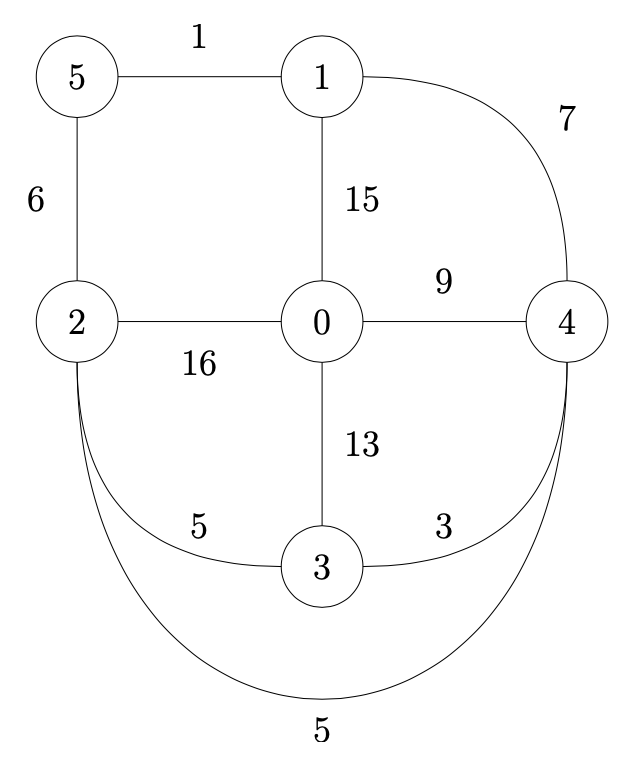
\includegraphics[width=0.3\textwidth]{../../Commun/Images/python-cours-graphe-dikstra.png}
\end{center}

\begin{itemize}
\item On commence à placer le sommet 0 dans la file avec la distance 0.
\item Le seul sommet de la file est le sommet 0. C'est donc celui dont
  la distance est minimale. On marque ce sommet comme visité puis on
  regarde ses voisins~: 1, 2, 3 et 4. On les place dans la file de priorité
  avec les distances respectives de 15, 16, 13 et 9.
\item Le sommet de la file ayant une distance minimale est 4. Cette distance est de 9.
  On le marque comme visité, puis on regarde ses voisins~: 1, 3 et 2.
  Le chemin passant par 4 et allant à 1 a une distance de 16 qui n'est pas inférieure
  à la distance actuelle pour 1. Par contre, le chemin passant par 4 et allant à 3
  a une distance de 12 qui est inférieure à la distance actuelle de 13 pour 3. C'est aussi le
  cas du chemin passant par 4 et allant à 2 dont la distance est 14. On met donc
  ces distances à jour dans notre file. Les sommets de la file sont donc désormais
  les sommets 1, 2, et 3 de distances respectives 15, 14 et 12.
\item Le sommet de la file ayant une distance minimale est 3. Cette distance est de 12.
  Aucun des chemins passant par 3 et menant à ses voisins ne permet d'obtenir une
  meilleure distance que celle que nous avons actuellement.
\item Le sommet de la file ayant une distance minimale est 2. 
  On marque ce sommet comme visité, puis on regarde ses voisins~: 4, 3, 0 et 5. La
  distance du sommet 2 étant 14, on insère donc le sommet 5 avec une distance de 20.
  Les sommets de la file sont désormais les sommets 1 et 5 de distances respectives 15 et 20.
\item Le sommet de la file ayant une distance minimale est 1. Cette distance est de 15.
  On marque ce sommet comme visité, puis on regarde ses voisins~: 0, 4 et 5.
  Le chemin passant par 1 et allant à 5 a une distance de 16 qui est inférieure
  à la distance temporaire de 20. On met donc à jour cette distance.
\item Le sommet de la file ayant une distance minimale est 5. Cette distance est de 16.
  On marque ce sommet comme visité. L'étude de ses voisins ne donne lieu à aucune mise à
  jour, car ils ont déjà tous été traités.
\item À la boucle suivante, il n'y a plus de sommet dans notre file et l'algorithme
  s'arrête. Les distances du sommet 0 aux autres sommets du graphe sont donc 0 pour 0,
  9 pour 4, 12 pour 3, 14 pour 2, 15 pour 1 et 16 pour 5.
\end{itemize}
\vspace{2ex}

Pour l'implémentation, nous utilisons le module \verb!heapq! de Python.

\begin{pythoncodeline}
import heapq

def dijkstra(g, s):
    """dijkstra(g: list[list[tuple[float, int]]], s: int) -> list[float]"""
    n = len(g)
    visite = [False for _ in range(n)]
    dist = [None for _ in range(n)]
    filep = []
    heapq.heappush(filep, (0.0, s))
    while len(filep) != 0:
        delta, x = heapq.heappop(filep)
        if not visite[x]:
            dist[x] = delta
            visite[x] = True
            for rho, y in g[x]:
                heapq.heappush(filep, (delta + rho, y))
    return dist
\end{pythoncodeline}

\vspace{2ex}
Si nous ne disposons pas de file de priorité, nous pouvons en faire une implémentation
à la main (qui ne sera malheureusement pas très efficace). Pour cela, nous allons utiliser
deux tableaux \emph{visité} et \emph{dist} dont la longueur est le nombre $n$ de sommets du graphe. Lorsqu'un sommet $x$ est dans l'état \emph{inconnu} c'est-à-dire lorsqu'il
n'a pas encore été inséré dans la liste, \verb!dist[x]! est égal à \verb!None! et
\verb!visite[x]! est égal à \verb!False!. Lorsqu'un sommet $x$ est dans la file,
\verb!dist[x]! contient sa priorité, et \verb!visite[x]! est égal à \verb!False!.
Enfin, lorsque $x$ est sorti de la file de priorité, \verb!dist[x]! contient la distance
de la source au sommet $x$ et \verb!visite[x]! est égal à \verb!True!.
On commence par écrire une fonction \verb!prochain_sommet! qui renvoie le sommet de
la file dont la distance est minimale.

\begin{pythoncodeline}
def prochain_sommet(dist, visite):
    """prochain_sommet(dist: list[float], visite: list[bool]) -> int"""
    n = len(dist)
    min_value = None
    min_x = None
    for x in range(n):
        if (not visite[x]) and (dist[x] != None) \
                and (min_value == None or dist[x] < min_value):
            min_value = dist[x]
            min_x = x
    return min_x
\end{pythoncodeline}
\noindent
L'algorithme de Dijkstra s'écrit alors naturellement.

\begin{pythoncodeline}
def dijkstra(g, s):
    """dijkstra(g: list[list[tuple[float, int]]], s: int) -> list[float]"""
    n = len(g)
    visite = [False for _ in range(n)]
    dist = [None for _ in range(n)]
    dist[s] = 0.0
    while True:
        x = prochain_sommet(dist, visite)
        if x == None:
            break
        visite[x] = True
        for rho, y in g[x]:
            delta = dist[x] + rho
            if dist[y] == None or delta < dist[y]:
                dist[y] = delta
    return dist
\end{pythoncodeline}

\subsubsection{Algorithme ${\rm A}^\star$}

L'algorithme de Dijkstra permet de déterminer la distance d'une source $s$ à
l'ensemble des sommets accessibles depuis $s$. Si l'on s'intéresse uniquement à la
distance entre la source et un but $b$, il est possible d'arrêter l'algorithme dès que
le sommet $b$ est
marqué comme visité. Sur la figure ci-dessous, on a réalisé une recherche du meilleur
chemin dans la ville d'Oldenburg, en Allemagne, en partant d'une source située en centre-ville et pour aller vers un but situé en périphérie, à l'ouest de la ville. Le chemin optimal trouvé est en rouge.

\begin{center}
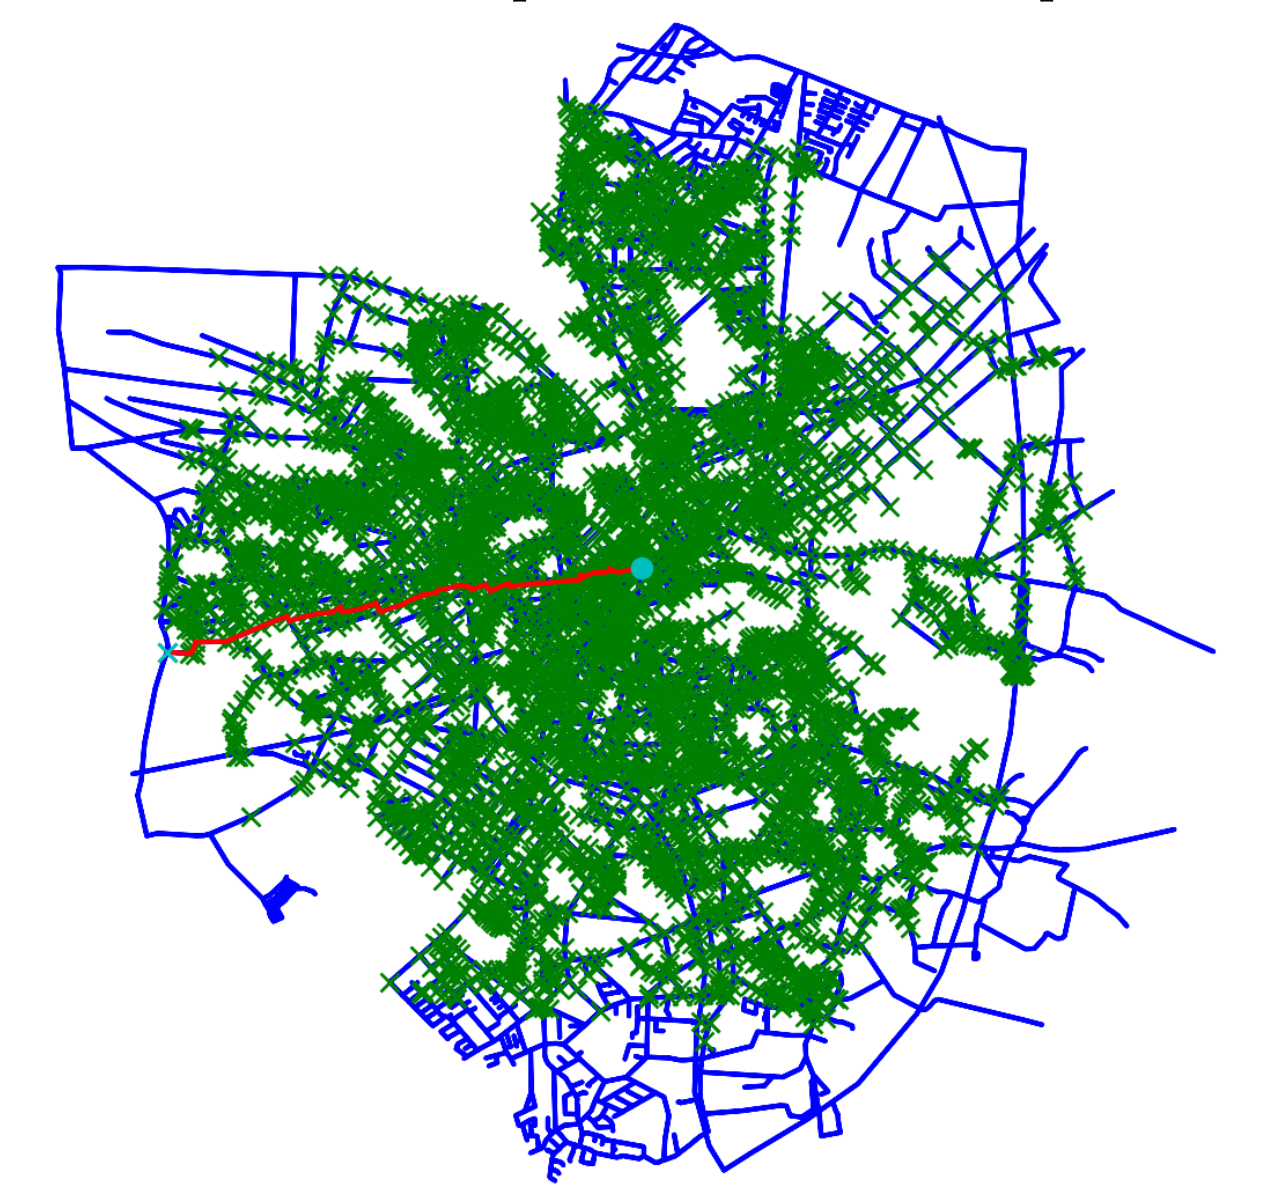
\includegraphics[width=0.4\textwidth]{../../Commun/Images/python-cours-graphe-astar-1.png}
\end{center}

Nous avons colorié en vert l'ensemble des sommets \og visités \fg par l'algorithme de
Dijkstra. La zone couverte par l'algorithme est formée de tous les points dont
la distance à la source est inférieure à la distance entre $s$ et $b$. Cependant, notre
intuition nous dit qu'il n'est surement pas utile d'aller traiter des sommets qui se
trouvent tout à l'est de la ville alors que notre but est à l'ouest. Cette intuition
se fonde sur le fait que la distance entre deux sommets $x$ et $y$ du graphe est
supérieure à la distance à vol d'oiseau entre ces deux sommets.\\

Pour exploiter cette idée, nous allons définir la fonction $h:S\to\R$, appelée
\emph{heuristique}, par
\[\forall x\in S\qsep h(x)\defeq\norme{x-b}\]
et définir une nouvelle distance $\rho'$ sur $A$ en définissant, pour tout
arc $x\to y$
\[\rho'(x\to y)=\rho(x\to y)+h(y)-h(x).\]
Remarquons tout d'abord que $\rho'$ est bien à valeurs positives puisque si $x\to y$ est
un arc
\[\rho(x\to y)\geq \norme{x-y}\geq \abs{\norme{x-b} - \norme{y-b}}\geq \norme{x-b} - \norme{y-b}=h(x)-h(y),\]
donc $\rho'(x\to y)=\rho(x\to y)+h(y)-h(x)\geq 0$. Remarquons enfin que, quel que
soit le chemin $z_0\to z_1\to\cdots\to z_n$, on a
$\rho'(z_0\to z_1\to\cdots\to z_n)=\rho(z_0\to z_1\to\cdots\to z_n)+h(z_n)-h(z_0)$.
En particulier
\[\rho'(s\to z_1\to\cdots\to z_{n-1}\to b)=\rho(s\to z_1\to\cdots\to z_{n-1}\to b)+h(b)-h(s).\]
Puisque $h(b)-h(s)$ est indépendant du chemin allant de $s$ à $b$,
tout chemin entre ces deux sommets de distance minimale pour $\rho'$ est minimal
pour $\rho$. L'algorithme de Dijkstra appliqué sur le même graphe
avec la distance $\rho'$ au lieu de la distance $\rho$ donnera donc un même chemin
minimal entre $s$ et $b$. Remarquons que cette nouvelle distance va privilégier les
sommets se situant en direction du but. En effet, dans le cas extrême où il existe
une ligne droite entre la source et le but et plusieurs sommets du graphe sont alignés,
la distance entre ces sommets pour la nouvelle distance $\rho'$ va être nulle et ce
sont bien ces sommets qui vont être traités en premier.\\

En reprenant la recherche du meilleur chemin entre le centre et un point de la périphérie
d'Oldenburg, on voit que l'algorithme de Dijkstra appliqué à
nouvelle distance traite beaucoup moins de sommets avant d'arriver sur le but, tout en garantissant le fait que
le chemin trouvé a une distance minimale pour la distance d'origine.

\begin{center}
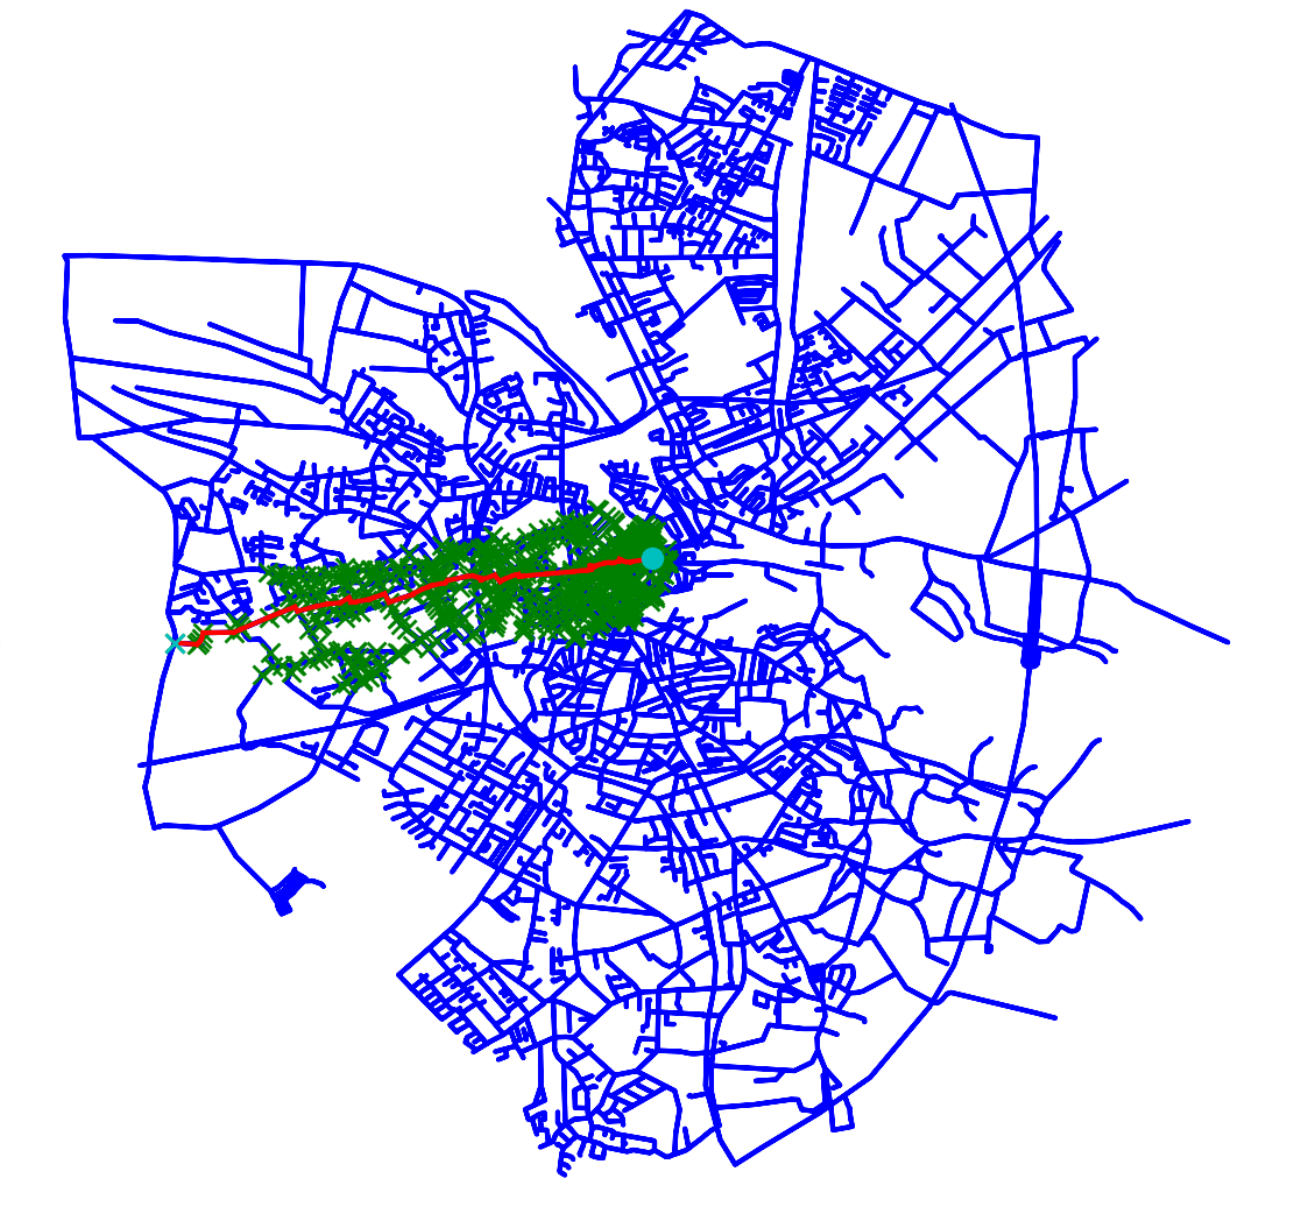
\includegraphics[width=0.4\textwidth]{../../Commun/Images/python-cours-graphe-astar-2.png}
\end{center}

%END_BOOK
\end{document}

